% ============================================================
% CARBON FIBER I-BEAM — SINGLE-PAGE PORTFOLIO CASE STUDY
% 01 Composites / Project 03
%
% IMPORTANT:
% 1. This file must NOT contain \documentclass, \begin{document},
%    or \end{document}.
% 2. In main.tex, place \input{ibeam_one_page} before \end{document}.
% 3. This script assumes the main portfolio preamble already defines:
%       DeepGreen, PolyGold, SoftGold, SoftGreen,
%       RuleGray, Muted, Ink
%    and loads tikz, graphicx, hyperref, and fontawesome5.
% 4. Upload these image files to Overleaf with the same names:
%       front view assembly graphic.png
%       Distributed weight with bolts.jpg
%       Stress Analysis on Generic CAD model.png
%       Beam Fiulure Delamination and cracking.jpeg
%       Three Point Bend Test.JPG
% ============================================================

\providecommand{\IBeamCompetitionGuidelines}
{https://drive.google.com/file/d/16S6MPVWWzPNKjXWVGKEySAi9i1f1BZYn/view?usp=sharing}

\providecommand{\IBeamBendTestVideo}
{https://drive.google.com/file/d/1LK_-pyK_y-a_4gDTiasz4uLUi95nAfrO/view?usp=drive_link}

\clearpage
\thispagestyle{empty}
\hypertarget{ibeam}{}
\null

\begin{tikzpicture}[remember picture,overlay]

% ============================================================
% BACKGROUND AND PAGE BARS
% ============================================================

\fill[white]
    (current page.south west)
    rectangle
    (current page.north east);

\fill[DeepGreen]
    (current page.north west)
    rectangle
    ($(current page.north east)+(0,-0.095in)$);

\fill[PolyGold]
    ($(current page.north west)+(0,-0.095in)$)
    rectangle
    ($(current page.north east)+(0,-0.14in)$);

\fill[DeepGreen]
    (current page.south west)
    rectangle
    ($(current page.south east)+(0,0.36in)$);

\fill[PolyGold]
    ($(current page.south west)+(0,0.36in)$)
    rectangle
    ($(current page.south east)+(0,0.405in)$);

% ============================================================
% HEADER
% ============================================================

\node[
    anchor=north west,
    text=PolyGold,
    font=\sffamily\bfseries\fontsize{8.1}{8.7}\selectfont
]
at ($(current page.north west)+(0.42in,-0.39in)$)
{01 COMPOSITES \hspace{5pt}/\hspace{5pt} PROJECT 03};

\node[
    anchor=north west,
    text=DeepGreen,
    font=\bfseries\fontsize{22.3}{23.3}\selectfont
]
at ($(current page.north west)+(0.40in,-0.67in)$)
{CARBON FIBER I-BEAM DESIGN \& TESTING};

\node[
    anchor=north west,
    text=Muted,
    font=\sffamily\fontsize{8.25}{9.0}\selectfont
]
at ($(current page.north west)+(0.42in,-1.12in)$)
{Cal Poly Composites Laboratory \hspace{7pt}\textbullet\hspace{7pt}
Individual Project \hspace{7pt}\textbullet\hspace{7pt}
Winter 2026 \hspace{7pt}\textbullet\hspace{7pt}
San Luis Obispo, California};

\fill[PolyGold]
    ($(current page.north west)+(0.42in,-1.36in)$)
    rectangle
    ($(current page.north west)+(6.10in,-1.315in)$);


% ============================================================
% TOP LEFT — ASSEMBLY ARCHITECTURE
% ============================================================

\node[
    anchor=north west,
    inner sep=2.6pt,
    draw=DeepGreen,
    line width=0.68pt,
    rounded corners=5pt
]
at ($(current page.north west)+(0.42in,-1.58in)$)
{
    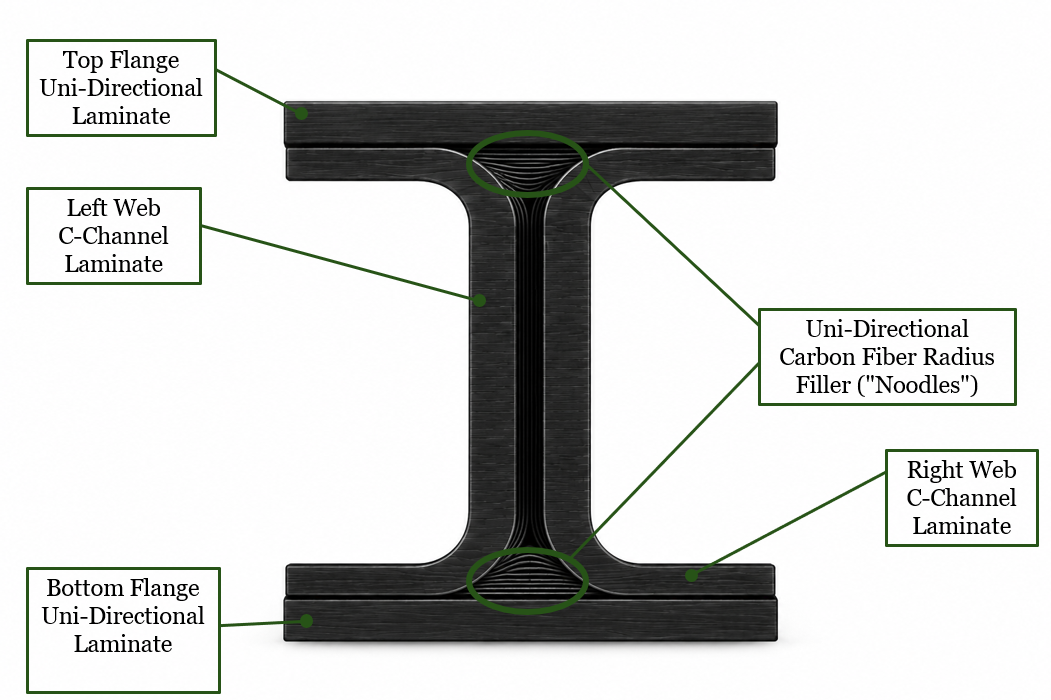
\includegraphics[
        width=3.55in,
        height=2.45in,
        keepaspectratio
    ]{front view assembly graphic.png}
};

\node[
    anchor=north,
    align=center,
    inner sep=0pt,
    text width=3.42in,
    text=Muted,
    font=\sffamily\fontsize{6.35}{7.05}\selectfont
]
at ($(current page.north west)+(2.195in,-4.12in)$)
{Four-piece laminate architecture with top and bottom flange laminates, paired C-channels, and longitudinal radius fillers};

% ============================================================
% TOP CENTER — PROJECT OVERVIEW + C-CHANNEL LAYUP
% ============================================================

\fill[SoftGold,rounded corners=5pt]
    ($(current page.north west)+(4.18in,-1.58in)$)
    rectangle
    ($(current page.north west)+(7.42in,-4.20in)$);

\fill[PolyGold]
    ($(current page.north west)+(4.18in,-1.58in)$)
    rectangle
    ($(current page.north west)+(4.28in,-4.20in)$);

\node[
    anchor=north west,
    text=DeepGreen,
    font=\sffamily\bfseries\fontsize{8.0}{8.7}\selectfont
]
at ($(current page.north west)+(4.48in,-1.76in)$)
{PROJECT OVERVIEW};

\node[
    anchor=north west,
    align=left,
    text width=2.64in,
    text=Ink,
    font=\fontsize{6.40}{7.45}\selectfont
]
at ($(current page.north west)+(4.48in,-2.04in)$)
{
A 24-inch carbon-fiber I-beam was manufactured from two molded
C-channel laminates, separate top and bottom flange laminates,
and longitudinal unidirectional radius fillers. The completed
684 g specimen sustained 28.2 kN (6,340 lbf) in three-point bending.\\[3pt]
\textbf{C-channel layup.}
Each channel used the same 12-ply sequence:
\mbox{$[+45/-45/0/+45/-45/0/0/-45/+45/0/-45/+45]$}.
The layup was completed twice, once for each channel.\\[3pt]
\textbf{Flange layups.}
Top flange: \mbox{$[90/0_6/90/0_6]$}. Bottom flange:
\mbox{$[90/0_6]$}, where $0_6$ denotes six consecutive 0-degree plies.
};

\node[
    anchor=south west,
    text=PolyGold,
    font=\sffamily\bfseries\fontsize{6.45}{7.1}\selectfont
]
at ($(current page.north west)+(4.48in,-4.03in)$)
{MASS: 684 g \hspace{8pt}\textbullet\hspace{8pt} PEAK LOAD: 28.2 kN \hspace{8pt}\textbullet\hspace{8pt} LENGTH: 24 in};

% ============================================================
% TOP RIGHT — C-CHANNEL MANUFACTURING
% ============================================================

\node[
    anchor=north west,
    inner sep=2.6pt,
    draw=DeepGreen,
    line width=0.68pt,
    rounded corners=5pt
]
at ($(current page.north west)+(7.62in,-1.58in)$)
{
    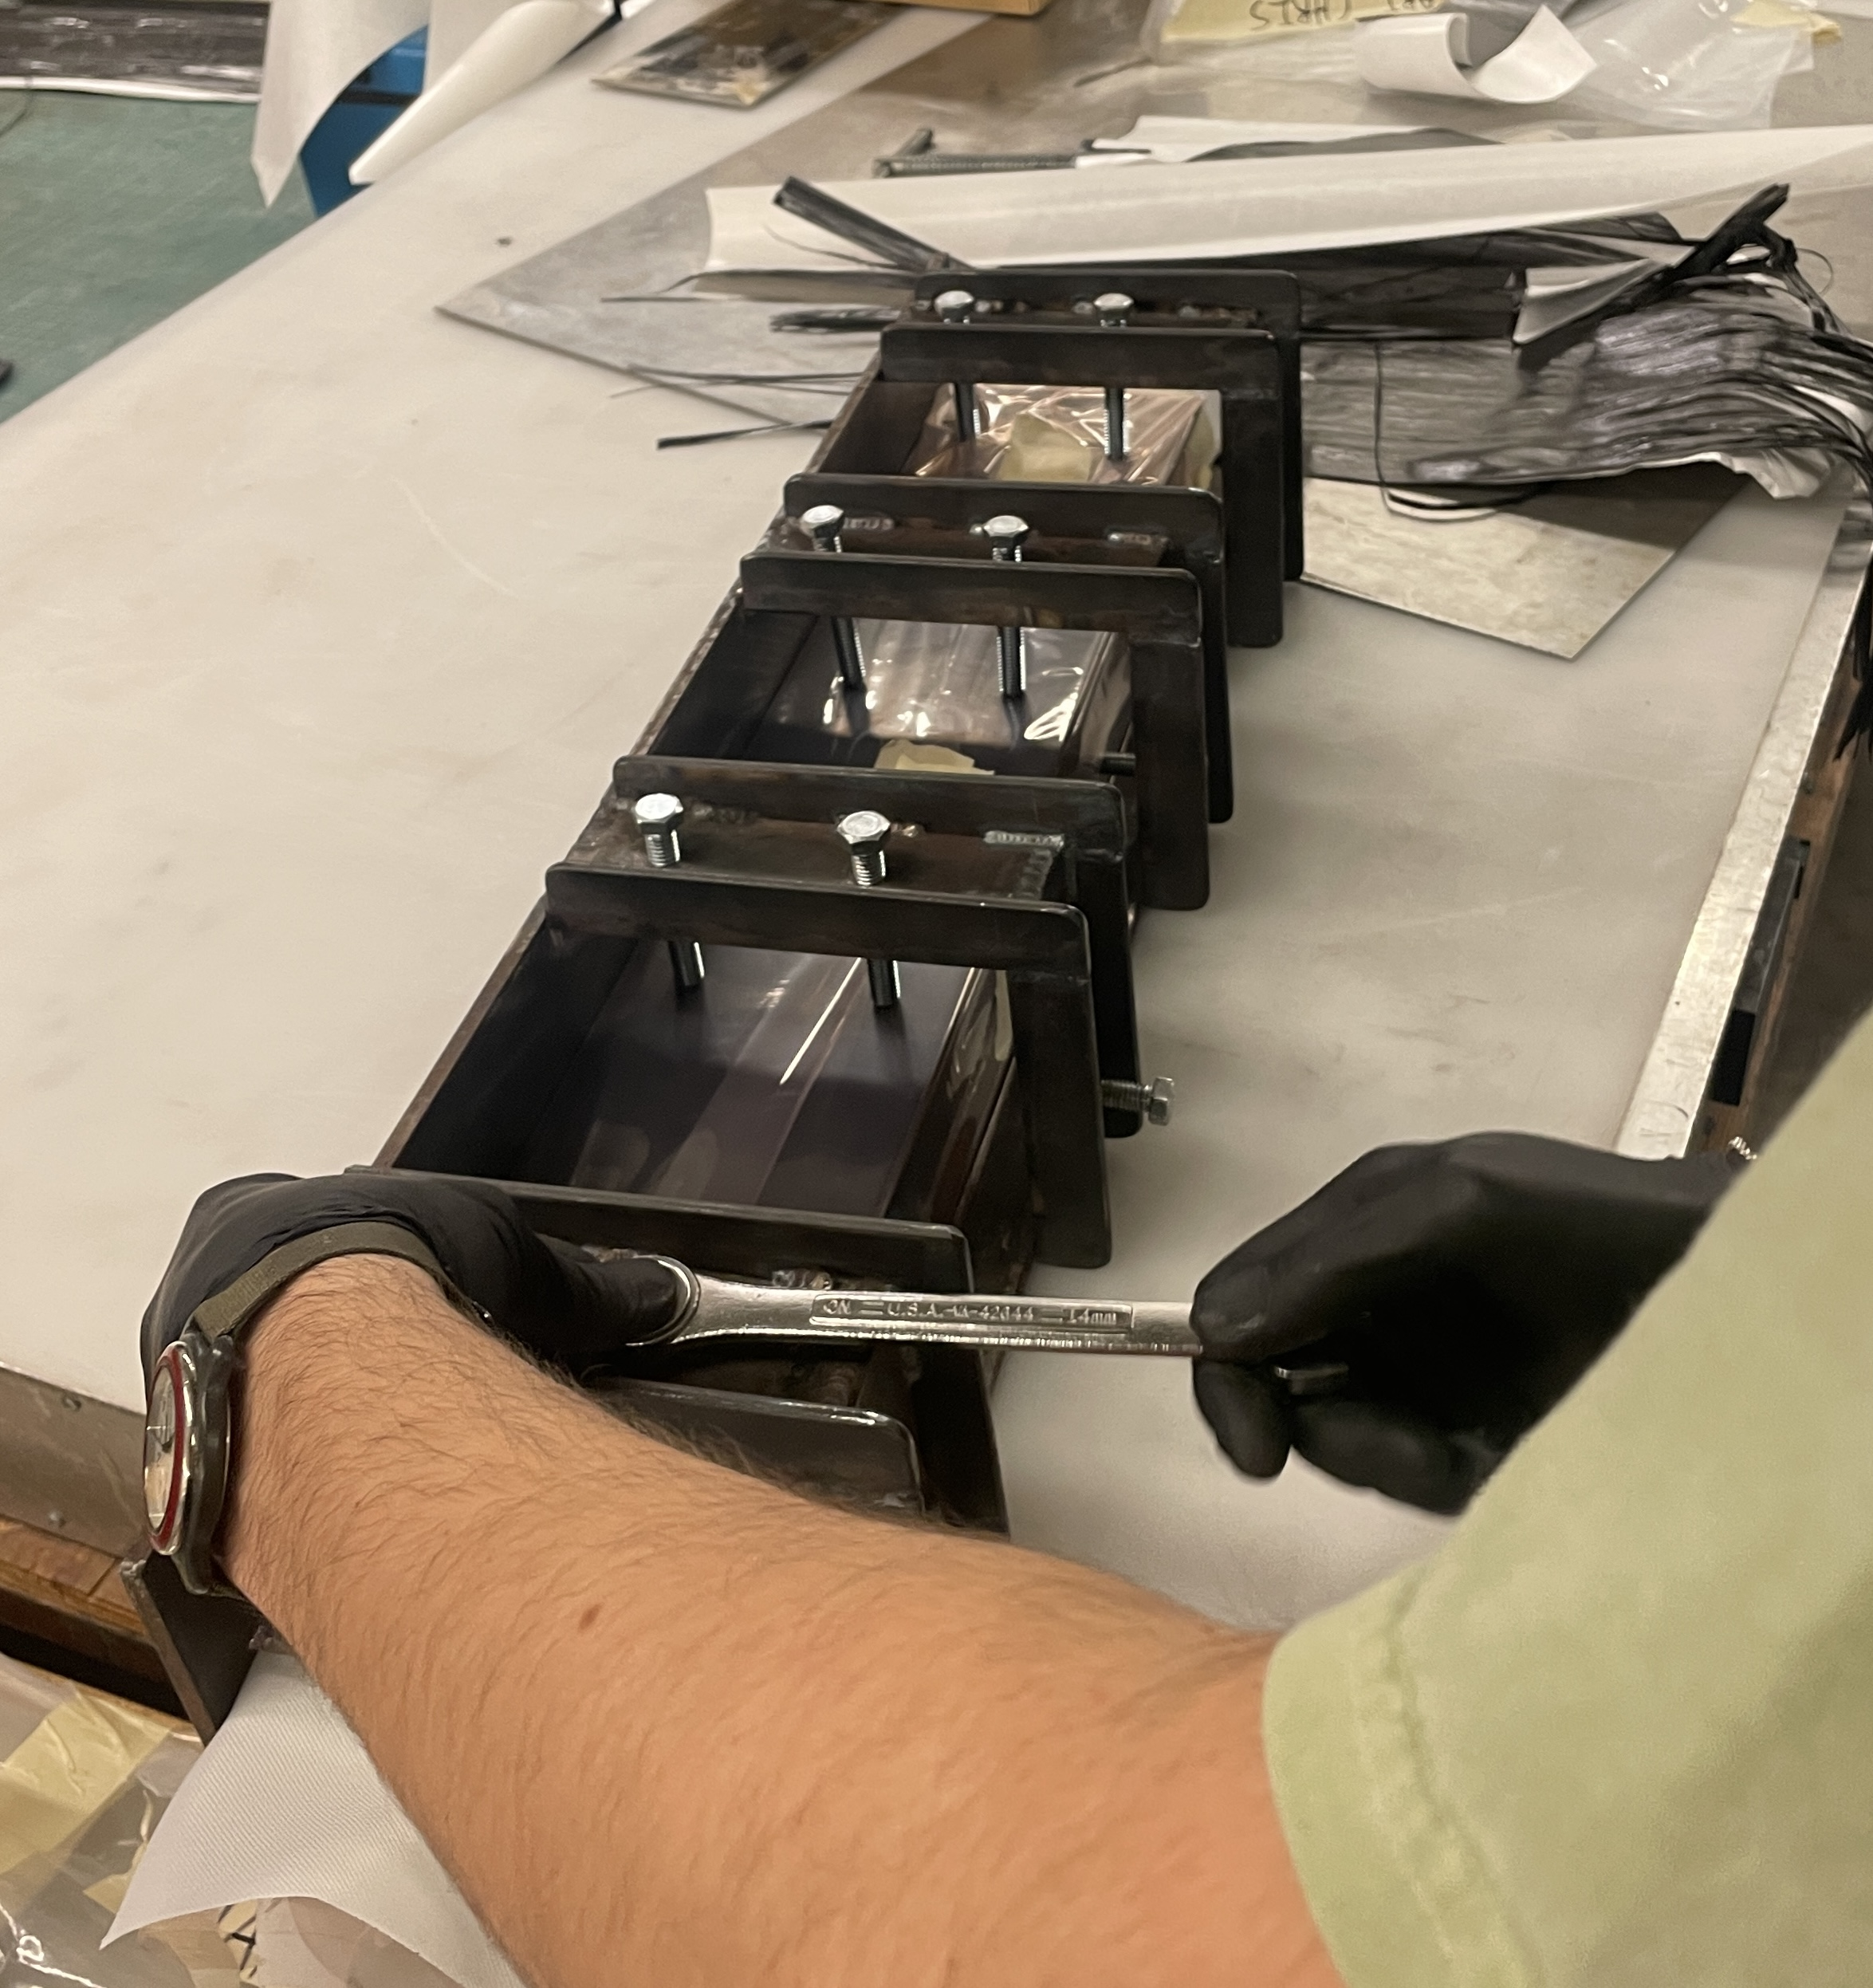
\includegraphics[
        width=3.55in,
        height=2.45in,
        keepaspectratio
    ]{Distributed weight with bolts.jpg}
};

\node[
    anchor=north,
    align=center,
    inner sep=0pt,
    text width=3.42in,
    text=Muted,
    font=\sffamily\fontsize{6.35}{7.05}\selectfont
]
at ($(current page.north west)+(9.395in,-4.12in)$)
{Distributed bolt pressure maintained alignment and consolidated the full beam assembly during cure};

% ============================================================
% CENTER ROW — MODEL, TEST, AND OBSERVED FAILURE
% ============================================================

\node[
    anchor=north west,
    inner sep=2.4pt,
    draw=RuleGray,
    line width=0.55pt,
    rounded corners=4pt
]
at ($(current page.north west)+(0.42in,-4.43in)$)
{
    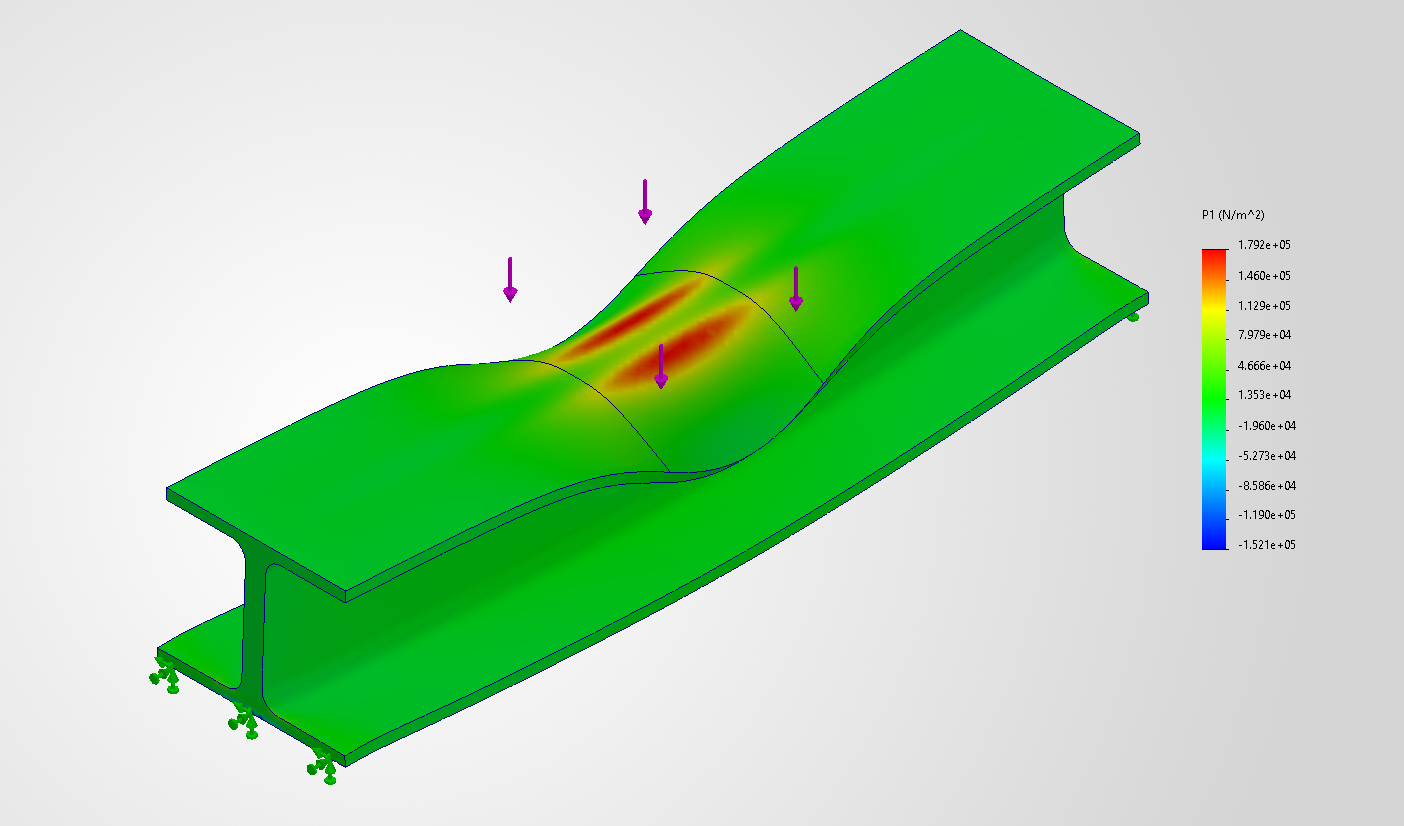
\includegraphics[
        width=3.33in,
        height=1.62in,
        keepaspectratio
    ]{Stress Analysis on Generic CAD model.png}
};

\node[
    anchor=north,
    align=center,
    inner sep=0pt,
    text width=3.20in,
    text=Muted,
    font=\sffamily\fontsize{6.20}{6.85}\selectfont
]
at ($(current page.north west)+(2.085in,-6.14in)$)
{Generic FEA predicted peak compressive stress beneath the center loading shoe};

\node[
    anchor=north west,
    inner sep=2.4pt,
    draw=RuleGray,
    line width=0.55pt,
    rounded corners=4pt
]
at ($(current page.north west)+(3.92in,-4.43in)$)
{
    \includegraphics[
        angle=180,
        origin=c,
        width=3.18in,
        height=1.62in,
        keepaspectratio
    ]{Three Point Bend Test.JPG}
};

\node[
    anchor=north,
    align=center,
    inner sep=0pt,
    text width=3.05in,
    text=Muted,
    font=\sffamily\fontsize{6.20}{6.85}\selectfont
]
at ($(current page.north west)+(5.510in,-6.14in)$)
{Experimental three-point bend test on the completed I-beam specimen};

\node[
    anchor=north west,
    inner sep=2.4pt,
    draw=RuleGray,
    line width=0.55pt,
    rounded corners=4pt
]
at ($(current page.north west)+(7.28in,-4.43in)$)
{
    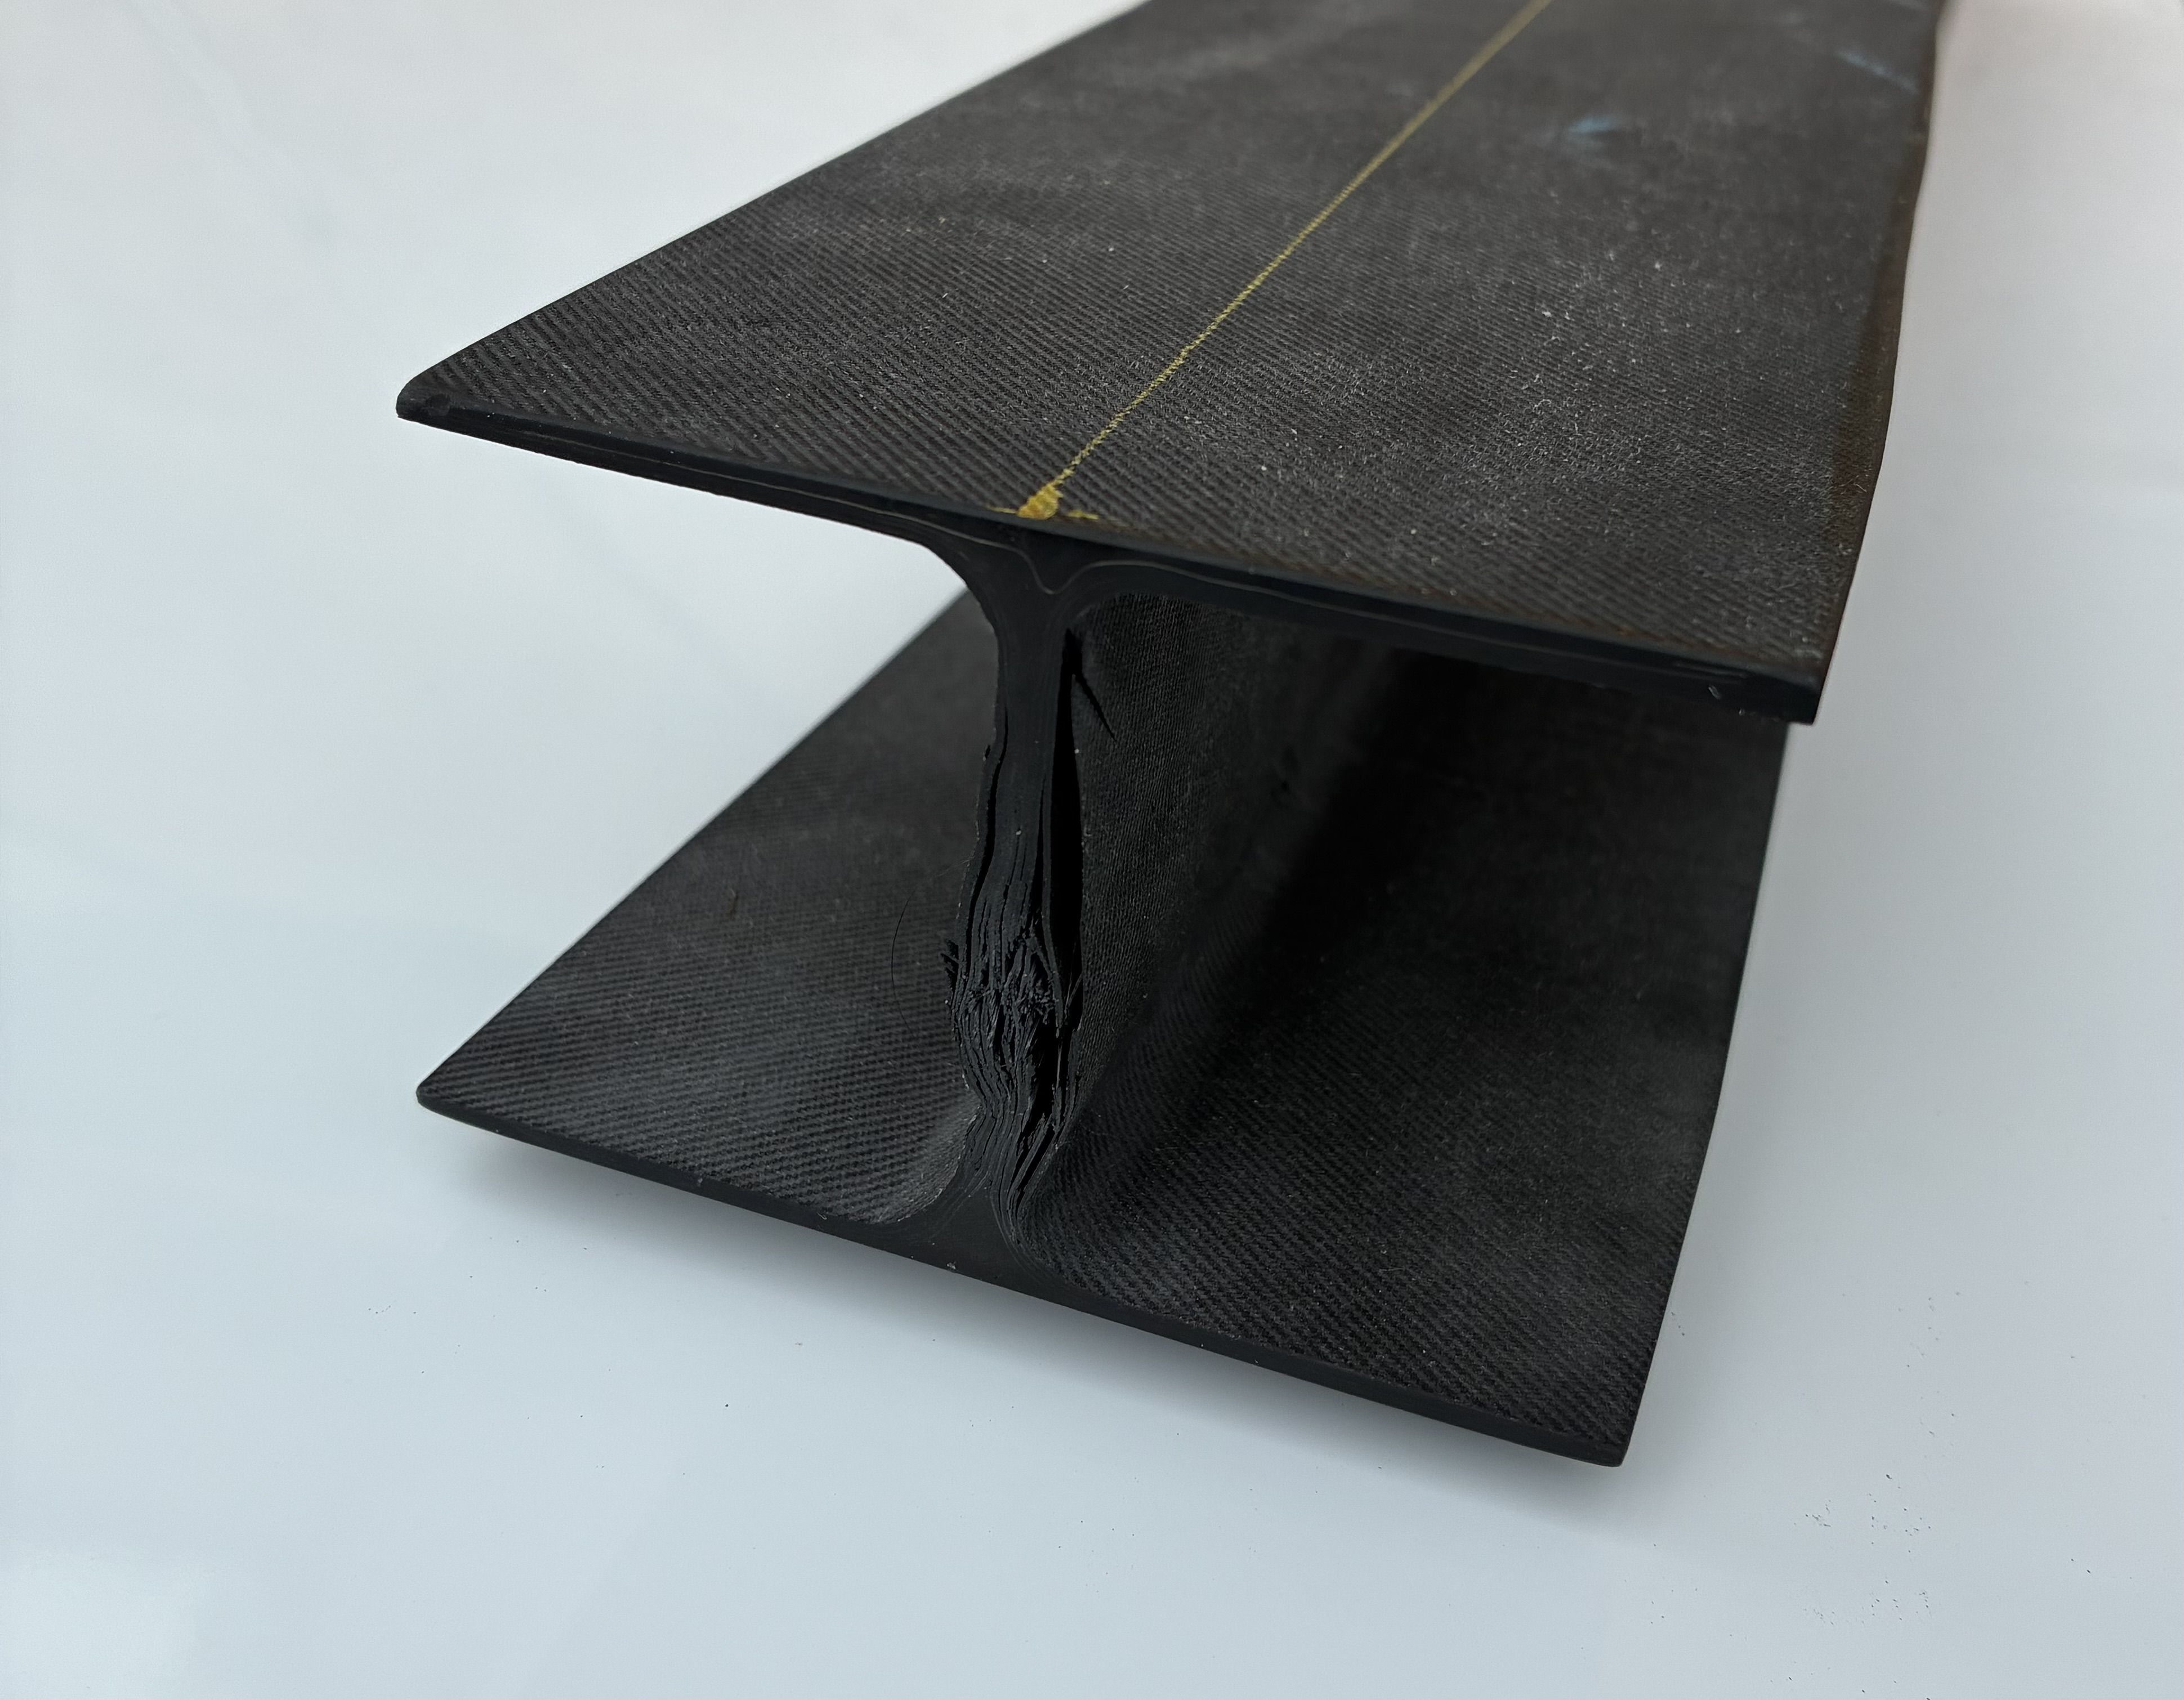
\includegraphics[
        width=3.65in,
        height=1.62in,
        keepaspectratio
    ]{Beam Fiulure Delamination and cracking.jpeg}
};

\node[
    anchor=north,
    align=center,
    inner sep=0pt,
    text width=3.50in,
    text=Muted,
    font=\sffamily\fontsize{6.20}{6.85}\selectfont
]
at ($(current page.north west)+(9.105in,-6.14in)$)
{Observed edge failure with delamination and longitudinal crack propagation};

% ============================================================
% BOTTOM LEFT — MANUFACTURING PROCESS
% ============================================================

\fill[SoftGreen,rounded corners=5pt]
    ($(current page.north west)+(0.42in,-6.43in)$)
    rectangle
    ($(current page.north west)+(5.30in,-7.18in)$);

\draw[RuleGray,line width=0.55pt,rounded corners=5pt]
    ($(current page.north west)+(0.42in,-6.43in)$)
    rectangle
    ($(current page.north west)+(5.30in,-7.18in)$);

\node[
    anchor=north west,
    text=DeepGreen,
    font=\sffamily\bfseries\fontsize{7.65}{8.35}\selectfont
]
at ($(current page.north west)+(0.66in,-6.57in)$)
{MANUFACTURING APPROACH};

\node[
    anchor=north west,
    align=left,
    text width=4.38in,
    text=Ink,
    font=\fontsize{6.20}{7.15}\selectfont
]
at ($(current page.north west)+(0.66in,-6.82in)$)
{
The separately molded channels were aligned with longitudinal carbon-fiber
``noodles'' filling the radius-induced flange voids. Top and bottom flanges
were then installed, and the full assembly was consolidated in a custom
steel fixture using distributed bolt pressure along the beam length.
};

% ============================================================
% BOTTOM RIGHT — FAILURE ANALYSIS AND NEXT ITERATION
% ============================================================

\fill[SoftGold,rounded corners=5pt]
    ($(current page.north west)+(5.52in,-6.43in)$)
    rectangle
    ($(current page.north east)+(-0.42in,-7.18in)$);

\fill[PolyGold]
    ($(current page.north west)+(5.52in,-6.43in)$)
    rectangle
    ($(current page.north west)+(5.62in,-7.18in)$);

\node[
    anchor=north west,
    text=DeepGreen,
    font=\sffamily\bfseries\fontsize{7.65}{8.35}\selectfont
]
at ($(current page.north west)+(5.82in,-6.57in)$)
{FAILURE ANALYSIS AND NEXT ITERATION};

\node[
    anchor=north west,
    align=left,
    text width=4.72in,
    text=Ink,
    font=\fontsize{6.14}{7.08}\selectfont
]
at ($(current page.north west)+(5.82in,-6.82in)$)
{
The model suggested a center-span compression failure, but the physical beam
failed near its edge. This mismatch indicates that local consolidation defects
likely enabled premature delamination. A future build should use staged vacuum
debulking after each ply group rather than relying only on manual rolling before
final fixture consolidation.
};

% ============================================================
% RESOURCE LINKS
% ============================================================

\node[
    anchor=north,
    align=center,
    text=DeepGreen,
    font=\sffamily\bfseries\fontsize{6.75}{7.35}\selectfont
]
at ($(current page.north)+(0,-7.43in)$)
{
\href{\IBeamCompetitionGuidelines}{\faFilePdf\ COMPETITION GUIDELINES}
\hspace{16pt}
\href{\IBeamBendTestVideo}{\faPlayCircle\ THREE-POINT BEND TEST VIDEO}
};

% ============================================================
% FOOTER
% ============================================================

\node[
    anchor=south west,
    text=white,
    font=\sffamily\bfseries\fontsize{7.1}{7.7}\selectfont
]
at ($(current page.south west)+(0.42in,0.17in)$)
{\hyperlink{pickleball}{\faArrowLeft\ PICKLEBALL PADDLE}};

\node[
    anchor=south,
    text=white,
    font=\sffamily\fontsize{7.0}{7.6}\selectfont
]
at ($(current page.south)+(0,0.17in)$)
{CARBON FIBER I-BEAM \hspace{6pt} 1 / 1};

\node[
    anchor=south east,
    text=white,
    font=\sffamily\bfseries\fontsize{7.1}{7.7}\selectfont
]
at ($(current page.south east)+(-0.42in,0.17in)$)
{NEXT PROJECT \faArrowRight};

\end{tikzpicture}
% ============================================================
% FIBERGLASS FUSELAGE FEA & THREE-POINT BEND VALIDATION
% SINGLE-PAGE PORTFOLIO CASE STUDY
% 01 Composites / Project 04
%
% IMPORTANT:
% 1. This file must NOT contain \documentclass, \begin{document},
%    or \end{document}.
% 2. In main.tex, place % ============================================================
% FIBERGLASS FUSELAGE FEA & THREE-POINT BEND VALIDATION
% SINGLE-PAGE PORTFOLIO CASE STUDY
% 01 Composites / Project 04
%
% IMPORTANT:
% 1. This file must NOT contain \documentclass, \begin{document},
%    or \end{document}.
% 2. In main.tex, place % ============================================================
% FIBERGLASS FUSELAGE FEA & THREE-POINT BEND VALIDATION
% SINGLE-PAGE PORTFOLIO CASE STUDY
% 01 Composites / Project 04
%
% IMPORTANT:
% 1. This file must NOT contain \documentclass, \begin{document},
%    or \end{document}.
% 2. In main.tex, place \input{fuselage} before \end{document}.
% 3. This script assumes the main portfolio preamble already defines:
%       DeepGreen, PolyGold, SoftGold, SoftGreen,
%       RuleGray, Muted, Ink
%    and loads tikz, graphicx, hyperref, and fontawesome5.
% 4. Upload these files to Overleaf with the exact same names:
%       Setup & Mesh of FEA.png
%       fuselage 3 point bend test.JPG
%       Countor Plot of Reaction Force.png
%       fuselage data.png
% ============================================================

\providecommand{\FuselageDemoVideo}
{https://drive.google.com/file/d/1xFCbBJXPhVVlnaleRyZeSM8ucD_xWwB2/view?usp=drive_link}

\providecommand{\FuselageFinalReport}
{https://drive.google.com/file/d/1LYRNlwk73l_KRgaSPgzfsYis-9bsuaxX/view?usp=drive_link}

\clearpage
\thispagestyle{empty}
\hypertarget{fuselage}{}
\null

\begin{tikzpicture}[remember picture,overlay]

% ============================================================
% BACKGROUND AND PAGE BARS
% ============================================================

\fill[white]
    (current page.south west)
    rectangle
    (current page.north east);

\fill[DeepGreen]
    (current page.north west)
    rectangle
    ($(current page.north east)+(0,-0.095in)$);

\fill[PolyGold]
    ($(current page.north west)+(0,-0.095in)$)
    rectangle
    ($(current page.north east)+(0,-0.14in)$);

\fill[DeepGreen]
    (current page.south west)
    rectangle
    ($(current page.south east)+(0,0.36in)$);

\fill[PolyGold]
    ($(current page.south west)+(0,0.36in)$)
    rectangle
    ($(current page.south east)+(0,0.405in)$);

% ============================================================
% HEADER
% ============================================================

\node[
    anchor=north west,
    text=PolyGold,
    font=\sffamily\bfseries\fontsize{8.1}{8.7}\selectfont
]
at ($(current page.north west)+(0.42in,-0.39in)$)
{01 COMPOSITES \hspace{5pt}/\hspace{5pt} PROJECT 04};

\node[
    anchor=north west,
    text=DeepGreen,
    font=\bfseries\fontsize{20.8}{21.8}\selectfont
]
at ($(current page.north west)+(0.40in,-0.67in)$)
{FIBERGLASS FUSELAGE FEA \& THREE-POINT BEND VALIDATION};

\node[
    anchor=north west,
    text=Muted,
    font=\sffamily\fontsize{8.15}{8.9}\selectfont
]
at ($(current page.north west)+(0.42in,-1.12in)$)
{Cal Poly Composites Laboratory \hspace{7pt}\textbullet\hspace{7pt}
Individual Project \hspace{7pt}\textbullet\hspace{7pt}
Winter 2026 \hspace{7pt}\textbullet\hspace{7pt}
San Luis Obispo, California};

\fill[PolyGold]
    ($(current page.north west)+(0.42in,-1.36in)$)
    rectangle
    ($(current page.north west)+(6.10in,-1.315in)$);


% ============================================================
% TOP LEFT — ABAQUS MODEL SETUP
% ============================================================

\node[
    anchor=north west,
    inner sep=2.6pt,
    draw=DeepGreen,
    line width=0.68pt,
    rounded corners=5pt
]
at ($(current page.north west)+(0.42in,-1.58in)$)
{
    \includegraphics[
        width=3.55in,
        height=2.34in,
        keepaspectratio
    ]{\detokenize{Setup & Mesh of FEA.png}}
};

\node[
    anchor=north,
    align=center,
    inner sep=0pt,
    text width=3.42in,
    text=Muted,
    font=\sffamily\fontsize{6.30}{7.00}\selectfont
]
at ($(current page.north west)+(2.195in,-4.02in)$)
{Abaqus assembly and quad-dominated mesh for the composite shell fuselage and rigid loading fixtures};

% ============================================================
% TOP CENTER — PROJECT OVERVIEW / STAR SUMMARY
% ============================================================

\fill[SoftGold,rounded corners=5pt]
    ($(current page.north west)+(4.18in,-1.58in)$)
    rectangle
    ($(current page.north west)+(8.55in,-4.10in)$);

\fill[PolyGold]
    ($(current page.north west)+(4.18in,-1.58in)$)
    rectangle
    ($(current page.north west)+(4.28in,-4.10in)$);

\node[
    anchor=north west,
    text=DeepGreen,
    font=\sffamily\bfseries\fontsize{8.0}{8.7}\selectfont
]
at ($(current page.north west)+(4.48in,-1.76in)$)
{PROJECT OVERVIEW};

\node[
    anchor=north west,
    align=left,
    text width=3.38in,
    text=Ink,
    font=\fontsize{6.28}{7.28}\selectfont
]
at ($(current page.north west)+(4.48in,-2.03in)$)
{
I developed and validated a seven-ply fiberglass fuselage model under a SAMPE-inspired three-point bend configuration. The Abaqus model reproduced the physical geometry, composite layup, rigid tooling, contact interactions, and displacement-controlled loading used during testing. I defined equivalent orthotropic lamina properties, preserved the 4-inch inner diameter through shell offset, created rigid-body reference points, and evaluated transverse-shear assumptions through sensitivity studies. The model correctly identified the experimentally observed critical region beneath the loading shoe, while the simulation-to-test comparison revealed the limitations of idealized composite failure modeling and guided a more defensible interpretation of the results.
};

\node[
    anchor=south west,
    text=PolyGold,
    font=\sffamily\bfseries\fontsize{6.35}{7.0}\selectfont
]
at ($(current page.north west)+(4.48in,-3.94in)$)
{7 PLIES \hspace{7pt}\textbullet\hspace{7pt} 20,584 SHELL ELEMENTS \hspace{7pt}\textbullet\hspace{7pt} 2 in DISPLACEMENT};

% ============================================================
% TOP RIGHT — PHYSICAL TEST
% ============================================================

\node[
    anchor=north west,
    inner sep=2.6pt,
    draw=DeepGreen,
    line width=0.68pt,
    rounded corners=5pt
]
at ($(current page.north west)+(8.70in,-1.58in)$)
{
    \includegraphics[
        angle=-90,
        origin=c,
        width=3.18in,
        height=2.18in,
        keepaspectratio
    ]{\detokenize{fuselage 3 point bend test.JPG}}
};

\node[
    anchor=north,
    align=center,
    inner sep=0pt,
    text width=2.70in,
    text=Muted,
    font=\sffamily\fontsize{6.30}{7.00}\selectfont
]
at ($(current page.north west)+(9.95in,-4.21in)$)
{Three-point bend validation test};

% ============================================================
% CENTER ROW — SIMULATION RESPONSE AND EXPERIMENTAL DATA
% ============================================================

% Left response card
\fill[SoftGreen!42,rounded corners=5pt]
    ($(current page.north west)+(0.42in,-4.34in)$)
    rectangle
    ($(current page.north west)+(6.60in,-6.28in)$);

\draw[RuleGray,line width=0.55pt,rounded corners=5pt]
    ($(current page.north west)+(0.42in,-4.34in)$)
    rectangle
    ($(current page.north west)+(5.55in,-6.28in)$);

\node[
    anchor=north west,
    text=DeepGreen,
    font=\sffamily\bfseries\fontsize{7.10}{7.75}\selectfont
]
at ($(current page.north west)+(0.66in,-4.48in)$)
{ABAQUS RESPONSE};

\node[
    anchor=north,
    inner sep=0pt
]
at ($(current page.north west)+(2.985in,-4.70in)$)
{
    \includegraphics[
        width=4.70in,
        height=1.26in,
        keepaspectratio
    ]{\detokenize{Countor Plot of Reaction Force.png}}
};

\node[
    anchor=north,
    align=center,
    inner sep=0pt,
    text width=4.55in,
    text=Muted,
    font=\sffamily\fontsize{6.15}{6.85}\selectfont
]
at ($(current page.north west)+(2.985in,-6.08in)$)
{Abaqus reaction-force response under bending};

% Right response card
\fill[SoftGreen!42,rounded corners=5pt]
    ($(current page.north west)+(5.76in,-4.34in)$)
    rectangle
    ($(current page.north east)+(-0.42in,-6.28in)$);

\draw[RuleGray,line width=0.55pt,rounded corners=5pt]
    ($(current page.north west)+(5.76in,-4.34in)$)
    rectangle
    ($(current page.north east)+(-0.42in,-6.28in)$);

\node[
    anchor=north west,
    text=DeepGreen,
    font=\sffamily\bfseries\fontsize{7.10}{7.75}\selectfont
]
at ($(current page.north west)+(6.00in,-4.48in)$)
{EXPERIMENTAL RESPONSE};

\node[
    anchor=north,
    inner sep=0pt
]
at ($(current page.north west)+(8.425in,-4.68in)$)
{
    \includegraphics[
        width=4.58in,
        height=1.32in,
        keepaspectratio
    ]{\detokenize{fuselage data.png}}
};

\node[
    anchor=north,
    align=center,
    inner sep=0pt,
    text width=4.45in,
    text=Muted,
    font=\sffamily\fontsize{6.15}{6.85}\selectfont
]
at ($(current page.north west)+(8.425in,-6.08in)$)
{Measured load history and peak response};

% ============================================================
% BOTTOM LEFT — MODELING APPROACH
% ============================================================

\fill[SoftGreen,rounded corners=5pt]
    ($(current page.north west)+(0.42in,-6.50in)$)
    rectangle
    ($(current page.north west)+(5.34in,-7.45in)$);

\draw[RuleGray,line width=0.55pt,rounded corners=5pt]
    ($(current page.north west)+(0.42in,-6.50in)$)
    rectangle
    ($(current page.north west)+(5.34in,-7.45in)$);

\node[
    anchor=north west,
    text=DeepGreen,
    font=\sffamily\bfseries\fontsize{7.65}{8.35}\selectfont
]
at ($(current page.north west)+(0.66in,-6.64in)$)
{MODELING APPROACH};

\node[
    anchor=north west,
    align=left,
    text width=4.44in,
    text=Ink,
    font=\fontsize{6.08}{7.02}\selectfont
]
at ($(current page.north west)+(0.66in,-6.89in)$)
{
The fuselage was represented as a seven-ply woven-fiberglass composite shell.
Rigid upper and lower fixtures transferred load through frictional contact, while
two static steps imposed 2 inches of total downward displacement. High- and
low-case studies for $G_{13}$ and $G_{23}$ changed peak reaction force by only
about 1.8\%, showing that the global response was not dominated by those assumptions.
};

% ============================================================
% BOTTOM RIGHT — VALIDATION AND ENGINEERING JUDGMENT
% ============================================================

\fill[SoftGold,rounded corners=5pt]
    ($(current page.north west)+(5.56in,-6.50in)$)
    rectangle
    ($(current page.north east)+(-0.42in,-7.45in)$);

\fill[PolyGold]
    ($(current page.north west)+(5.56in,-6.50in)$)
    rectangle
    ($(current page.north west)+(5.66in,-7.45in)$);

\node[
    anchor=north west,
    text=DeepGreen,
    font=\sffamily\bfseries\fontsize{7.65}{8.35}\selectfont
]
at ($(current page.north west)+(5.86in,-6.64in)$)
{VALIDATION AND ENGINEERING JUDGMENT};

\node[
    anchor=north west,
    align=left,
    text width=4.66in,
    text=Ink,
    font=\fontsize{6.02}{6.96}\selectfont
]
at ($(current page.north west)+(5.86in,-6.89in)$)
{
Abaqus predicted 1,814 lbf versus the measured 1,123.82 lbf, an overprediction
of 61.4\%. Rather than treating the model as fully validated, I traced the gap to
approximated material properties, idealized shell geometry, simplified contact,
and the absence of progressive crushing, delamination, and tear-through.
The study demonstrated both technical persistence and the judgment to distinguish
useful qualitative agreement from unsupported quantitative confidence.
};

% ============================================================
% RESOURCE LINKS
% ============================================================

\node[
    anchor=north,
    align=center,
    text=DeepGreen,
    font=\sffamily\bfseries\fontsize{6.75}{7.35}\selectfont
]
at ($(current page.north)+(0,-7.56in)$)
{
\href{\FuselageFinalReport}{\faFilePdf\ FINAL ANALYSIS REPORT}
\hspace{16pt}
\href{\FuselageDemoVideo}{\faPlayCircle\ FUSELAGE DEMONSTRATION}
};

% ============================================================
% FOOTER
% ============================================================

\node[
    anchor=south west,
    text=white,
    font=\sffamily\bfseries\fontsize{7.1}{7.7}\selectfont
]
at ($(current page.south west)+(0.42in,0.17in)$)
{\hyperlink{ibeam}{\faArrowLeft\ CARBON FIBER I-BEAM}};

\node[
    anchor=south,
    text=white,
    font=\sffamily\fontsize{7.0}{7.6}\selectfont
]
at ($(current page.south)+(0,0.17in)$)
{FIBERGLASS FUSELAGE \hspace{6pt} 1 / 1};

\node[
    anchor=south east,
    text=white,
    font=\sffamily\bfseries\fontsize{7.1}{7.7}\selectfont
]
at ($(current page.south east)+(-0.42in,0.17in)$)
{NEXT PROJECT \faArrowRight};

\end{tikzpicture}
\input{coupons}
\clearpage
 before \end{document}.
% 3. This script assumes the main portfolio preamble already defines:
%       DeepGreen, PolyGold, SoftGold, SoftGreen,
%       RuleGray, Muted, Ink
%    and loads tikz, graphicx, hyperref, and fontawesome5.
% 4. Upload these files to Overleaf with the exact same names:
%       Setup & Mesh of FEA.png
%       fuselage 3 point bend test.JPG
%       Countor Plot of Reaction Force.png
%       fuselage data.png
% ============================================================

\providecommand{\FuselageDemoVideo}
{https://drive.google.com/file/d/1xFCbBJXPhVVlnaleRyZeSM8ucD_xWwB2/view?usp=drive_link}

\providecommand{\FuselageFinalReport}
{https://drive.google.com/file/d/1LYRNlwk73l_KRgaSPgzfsYis-9bsuaxX/view?usp=drive_link}

\clearpage
\thispagestyle{empty}
\hypertarget{fuselage}{}
\null

\begin{tikzpicture}[remember picture,overlay]

% ============================================================
% BACKGROUND AND PAGE BARS
% ============================================================

\fill[white]
    (current page.south west)
    rectangle
    (current page.north east);

\fill[DeepGreen]
    (current page.north west)
    rectangle
    ($(current page.north east)+(0,-0.095in)$);

\fill[PolyGold]
    ($(current page.north west)+(0,-0.095in)$)
    rectangle
    ($(current page.north east)+(0,-0.14in)$);

\fill[DeepGreen]
    (current page.south west)
    rectangle
    ($(current page.south east)+(0,0.36in)$);

\fill[PolyGold]
    ($(current page.south west)+(0,0.36in)$)
    rectangle
    ($(current page.south east)+(0,0.405in)$);

% ============================================================
% HEADER
% ============================================================

\node[
    anchor=north west,
    text=PolyGold,
    font=\sffamily\bfseries\fontsize{8.1}{8.7}\selectfont
]
at ($(current page.north west)+(0.42in,-0.39in)$)
{01 COMPOSITES \hspace{5pt}/\hspace{5pt} PROJECT 04};

\node[
    anchor=north west,
    text=DeepGreen,
    font=\bfseries\fontsize{20.8}{21.8}\selectfont
]
at ($(current page.north west)+(0.40in,-0.67in)$)
{FIBERGLASS FUSELAGE FEA \& THREE-POINT BEND VALIDATION};

\node[
    anchor=north west,
    text=Muted,
    font=\sffamily\fontsize{8.15}{8.9}\selectfont
]
at ($(current page.north west)+(0.42in,-1.12in)$)
{Cal Poly Composites Laboratory \hspace{7pt}\textbullet\hspace{7pt}
Individual Project \hspace{7pt}\textbullet\hspace{7pt}
Winter 2026 \hspace{7pt}\textbullet\hspace{7pt}
San Luis Obispo, California};

\fill[PolyGold]
    ($(current page.north west)+(0.42in,-1.36in)$)
    rectangle
    ($(current page.north west)+(6.10in,-1.315in)$);


% ============================================================
% TOP LEFT — ABAQUS MODEL SETUP
% ============================================================

\node[
    anchor=north west,
    inner sep=2.6pt,
    draw=DeepGreen,
    line width=0.68pt,
    rounded corners=5pt
]
at ($(current page.north west)+(0.42in,-1.58in)$)
{
    \includegraphics[
        width=3.55in,
        height=2.34in,
        keepaspectratio
    ]{\detokenize{Setup & Mesh of FEA.png}}
};

\node[
    anchor=north,
    align=center,
    inner sep=0pt,
    text width=3.42in,
    text=Muted,
    font=\sffamily\fontsize{6.30}{7.00}\selectfont
]
at ($(current page.north west)+(2.195in,-4.02in)$)
{Abaqus assembly and quad-dominated mesh for the composite shell fuselage and rigid loading fixtures};

% ============================================================
% TOP CENTER — PROJECT OVERVIEW / STAR SUMMARY
% ============================================================

\fill[SoftGold,rounded corners=5pt]
    ($(current page.north west)+(4.18in,-1.58in)$)
    rectangle
    ($(current page.north west)+(8.55in,-4.10in)$);

\fill[PolyGold]
    ($(current page.north west)+(4.18in,-1.58in)$)
    rectangle
    ($(current page.north west)+(4.28in,-4.10in)$);

\node[
    anchor=north west,
    text=DeepGreen,
    font=\sffamily\bfseries\fontsize{8.0}{8.7}\selectfont
]
at ($(current page.north west)+(4.48in,-1.76in)$)
{PROJECT OVERVIEW};

\node[
    anchor=north west,
    align=left,
    text width=3.38in,
    text=Ink,
    font=\fontsize{6.28}{7.28}\selectfont
]
at ($(current page.north west)+(4.48in,-2.03in)$)
{
I developed and validated a seven-ply fiberglass fuselage model under a SAMPE-inspired three-point bend configuration. The Abaqus model reproduced the physical geometry, composite layup, rigid tooling, contact interactions, and displacement-controlled loading used during testing. I defined equivalent orthotropic lamina properties, preserved the 4-inch inner diameter through shell offset, created rigid-body reference points, and evaluated transverse-shear assumptions through sensitivity studies. The model correctly identified the experimentally observed critical region beneath the loading shoe, while the simulation-to-test comparison revealed the limitations of idealized composite failure modeling and guided a more defensible interpretation of the results.
};

\node[
    anchor=south west,
    text=PolyGold,
    font=\sffamily\bfseries\fontsize{6.35}{7.0}\selectfont
]
at ($(current page.north west)+(4.48in,-3.94in)$)
{7 PLIES \hspace{7pt}\textbullet\hspace{7pt} 20,584 SHELL ELEMENTS \hspace{7pt}\textbullet\hspace{7pt} 2 in DISPLACEMENT};

% ============================================================
% TOP RIGHT — PHYSICAL TEST
% ============================================================

\node[
    anchor=north west,
    inner sep=2.6pt,
    draw=DeepGreen,
    line width=0.68pt,
    rounded corners=5pt
]
at ($(current page.north west)+(8.70in,-1.58in)$)
{
    \includegraphics[
        angle=-90,
        origin=c,
        width=3.18in,
        height=2.18in,
        keepaspectratio
    ]{\detokenize{fuselage 3 point bend test.JPG}}
};

\node[
    anchor=north,
    align=center,
    inner sep=0pt,
    text width=2.70in,
    text=Muted,
    font=\sffamily\fontsize{6.30}{7.00}\selectfont
]
at ($(current page.north west)+(9.95in,-4.21in)$)
{Three-point bend validation test};

% ============================================================
% CENTER ROW — SIMULATION RESPONSE AND EXPERIMENTAL DATA
% ============================================================

% Left response card
\fill[SoftGreen!42,rounded corners=5pt]
    ($(current page.north west)+(0.42in,-4.34in)$)
    rectangle
    ($(current page.north west)+(6.60in,-6.28in)$);

\draw[RuleGray,line width=0.55pt,rounded corners=5pt]
    ($(current page.north west)+(0.42in,-4.34in)$)
    rectangle
    ($(current page.north west)+(5.55in,-6.28in)$);

\node[
    anchor=north west,
    text=DeepGreen,
    font=\sffamily\bfseries\fontsize{7.10}{7.75}\selectfont
]
at ($(current page.north west)+(0.66in,-4.48in)$)
{ABAQUS RESPONSE};

\node[
    anchor=north,
    inner sep=0pt
]
at ($(current page.north west)+(2.985in,-4.70in)$)
{
    \includegraphics[
        width=4.70in,
        height=1.26in,
        keepaspectratio
    ]{\detokenize{Countor Plot of Reaction Force.png}}
};

\node[
    anchor=north,
    align=center,
    inner sep=0pt,
    text width=4.55in,
    text=Muted,
    font=\sffamily\fontsize{6.15}{6.85}\selectfont
]
at ($(current page.north west)+(2.985in,-6.08in)$)
{Abaqus reaction-force response under bending};

% Right response card
\fill[SoftGreen!42,rounded corners=5pt]
    ($(current page.north west)+(5.76in,-4.34in)$)
    rectangle
    ($(current page.north east)+(-0.42in,-6.28in)$);

\draw[RuleGray,line width=0.55pt,rounded corners=5pt]
    ($(current page.north west)+(5.76in,-4.34in)$)
    rectangle
    ($(current page.north east)+(-0.42in,-6.28in)$);

\node[
    anchor=north west,
    text=DeepGreen,
    font=\sffamily\bfseries\fontsize{7.10}{7.75}\selectfont
]
at ($(current page.north west)+(6.00in,-4.48in)$)
{EXPERIMENTAL RESPONSE};

\node[
    anchor=north,
    inner sep=0pt
]
at ($(current page.north west)+(8.425in,-4.68in)$)
{
    \includegraphics[
        width=4.58in,
        height=1.32in,
        keepaspectratio
    ]{\detokenize{fuselage data.png}}
};

\node[
    anchor=north,
    align=center,
    inner sep=0pt,
    text width=4.45in,
    text=Muted,
    font=\sffamily\fontsize{6.15}{6.85}\selectfont
]
at ($(current page.north west)+(8.425in,-6.08in)$)
{Measured load history and peak response};

% ============================================================
% BOTTOM LEFT — MODELING APPROACH
% ============================================================

\fill[SoftGreen,rounded corners=5pt]
    ($(current page.north west)+(0.42in,-6.50in)$)
    rectangle
    ($(current page.north west)+(5.34in,-7.45in)$);

\draw[RuleGray,line width=0.55pt,rounded corners=5pt]
    ($(current page.north west)+(0.42in,-6.50in)$)
    rectangle
    ($(current page.north west)+(5.34in,-7.45in)$);

\node[
    anchor=north west,
    text=DeepGreen,
    font=\sffamily\bfseries\fontsize{7.65}{8.35}\selectfont
]
at ($(current page.north west)+(0.66in,-6.64in)$)
{MODELING APPROACH};

\node[
    anchor=north west,
    align=left,
    text width=4.44in,
    text=Ink,
    font=\fontsize{6.08}{7.02}\selectfont
]
at ($(current page.north west)+(0.66in,-6.89in)$)
{
The fuselage was represented as a seven-ply woven-fiberglass composite shell.
Rigid upper and lower fixtures transferred load through frictional contact, while
two static steps imposed 2 inches of total downward displacement. High- and
low-case studies for $G_{13}$ and $G_{23}$ changed peak reaction force by only
about 1.8\%, showing that the global response was not dominated by those assumptions.
};

% ============================================================
% BOTTOM RIGHT — VALIDATION AND ENGINEERING JUDGMENT
% ============================================================

\fill[SoftGold,rounded corners=5pt]
    ($(current page.north west)+(5.56in,-6.50in)$)
    rectangle
    ($(current page.north east)+(-0.42in,-7.45in)$);

\fill[PolyGold]
    ($(current page.north west)+(5.56in,-6.50in)$)
    rectangle
    ($(current page.north west)+(5.66in,-7.45in)$);

\node[
    anchor=north west,
    text=DeepGreen,
    font=\sffamily\bfseries\fontsize{7.65}{8.35}\selectfont
]
at ($(current page.north west)+(5.86in,-6.64in)$)
{VALIDATION AND ENGINEERING JUDGMENT};

\node[
    anchor=north west,
    align=left,
    text width=4.66in,
    text=Ink,
    font=\fontsize{6.02}{6.96}\selectfont
]
at ($(current page.north west)+(5.86in,-6.89in)$)
{
Abaqus predicted 1,814 lbf versus the measured 1,123.82 lbf, an overprediction
of 61.4\%. Rather than treating the model as fully validated, I traced the gap to
approximated material properties, idealized shell geometry, simplified contact,
and the absence of progressive crushing, delamination, and tear-through.
The study demonstrated both technical persistence and the judgment to distinguish
useful qualitative agreement from unsupported quantitative confidence.
};

% ============================================================
% RESOURCE LINKS
% ============================================================

\node[
    anchor=north,
    align=center,
    text=DeepGreen,
    font=\sffamily\bfseries\fontsize{6.75}{7.35}\selectfont
]
at ($(current page.north)+(0,-7.56in)$)
{
\href{\FuselageFinalReport}{\faFilePdf\ FINAL ANALYSIS REPORT}
\hspace{16pt}
\href{\FuselageDemoVideo}{\faPlayCircle\ FUSELAGE DEMONSTRATION}
};

% ============================================================
% FOOTER
% ============================================================

\node[
    anchor=south west,
    text=white,
    font=\sffamily\bfseries\fontsize{7.1}{7.7}\selectfont
]
at ($(current page.south west)+(0.42in,0.17in)$)
{\hyperlink{ibeam}{\faArrowLeft\ CARBON FIBER I-BEAM}};

\node[
    anchor=south,
    text=white,
    font=\sffamily\fontsize{7.0}{7.6}\selectfont
]
at ($(current page.south)+(0,0.17in)$)
{FIBERGLASS FUSELAGE \hspace{6pt} 1 / 1};

\node[
    anchor=south east,
    text=white,
    font=\sffamily\bfseries\fontsize{7.1}{7.7}\selectfont
]
at ($(current page.south east)+(-0.42in,0.17in)$)
{NEXT PROJECT \faArrowRight};

\end{tikzpicture}
% ============================================================
% CARBON FIBER LAMINA MANUFACTURING & TENSILE CHARACTERIZATION
% TWO-PAGE PORTFOLIO CASE STUDY
% 01 Composites / Project 05
%
% IMPORTANT:
% 1. This file must NOT contain \documentclass, \begin{document},
%    or \end{document}.
% 2. In main.tex, place \input{coupon_testing} before \end{document}.
% 3. This script assumes the main portfolio preamble already defines:
%       DeepGreen, PolyGold, SoftGold, SoftGreen,
%       RuleGray, Muted, Ink
%    and loads tikz, graphicx, hyperref, and fontawesome5.
% 4. Upload these files to Overleaf with the exact same names:
%       Lamina Layering.png
%       Lamina Layer Rolling.JPG
%       Vacuum Bagging Panels.png
%       Autoclave.png
%       Cutting Coupon Samples.png
%       Catastrophic Laminate Failure.JPG
%       Stress Strain Plot.png
%       Q bar.png
%       S bar.png
% ============================================================

\providecommand{\CouponFailureVideo}
{https://drive.google.com/file/d/1EytOiadSSdiBPm855tiwnkO2kXlO5trU/view?usp=drive_link}

\providecommand{\CouponReportOne}
{https://drive.google.com/file/d/1XtEZSRZMTFmzKIk3v_zTwT6gxZyLEyW5/view?usp=sharing}

\providecommand{\CouponReportTwo}
{https://drive.google.com/file/d/1dq82_FQC8oGFbILCtTh4ZzD-SmT6Ute4/view?usp=drive_link}

\providecommand{\CouponReportThree}
{https://drive.google.com/file/d/1Gu54UFZfrPYRrOnVh5Dqf-ldtvUttEf5/view?usp=drive_link}

% ============================================================
% PAGE 1 — MANUFACTURING
% ============================================================

\clearpage
\thispagestyle{empty}
\hypertarget{coupon-testing}{}
\null

\begin{tikzpicture}[remember picture,overlay]

% PAGE BACKGROUND AND BARS
\fill[white] (current page.south west) rectangle (current page.north east);
\fill[DeepGreen] (current page.north west) rectangle ($(current page.north east)+(0,-0.095in)$);
\fill[PolyGold] ($(current page.north west)+(0,-0.095in)$) rectangle ($(current page.north east)+(0,-0.14in)$);
\fill[DeepGreen] (current page.south west) rectangle ($(current page.south east)+(0,0.36in)$);
\fill[PolyGold] ($(current page.south west)+(0,0.36in)$) rectangle ($(current page.south east)+(0,0.405in)$);

% HEADER
\node[anchor=north west,text=PolyGold,font=\sffamily\bfseries\fontsize{8.1}{8.7}\selectfont]
at ($(current page.north west)+(0.42in,-0.39in)$)
{01 COMPOSITES \hspace{5pt}/\hspace{5pt} PROJECT 05};

\node[anchor=north west,text=DeepGreen,font=\bfseries\fontsize{17.6}{18.7}\selectfont]
at ($(current page.north west)+(0.40in,-0.67in)$)
{CARBON FIBER COUPON MANUFACTURING \& TENSILE TESTING};

\node[anchor=north west,text=Muted,font=\sffamily\fontsize{8.15}{8.9}\selectfont]
at ($(current page.north west)+(0.42in,-1.12in)$)
{Cal Poly Composites Laboratory \hspace{7pt}\textbullet\hspace{7pt}
Team Project \hspace{7pt}\textbullet\hspace{7pt}
Summer 2025 \hspace{7pt}\textbullet\hspace{7pt}
San Luis Obispo, California};

\fill[PolyGold]
    ($(current page.north west)+(0.42in,-1.36in)$)
    rectangle
    ($(current page.north west)+(6.10in,-1.315in)$);


% OVERVIEW — LEFT COLUMN
\fill[SoftGold,rounded corners=5pt]
($(current page.north west)+(0.42in,-1.58in)$) rectangle ($(current page.north west)+(3.18in,-6.22in)$);
\fill[PolyGold]
($(current page.north west)+(0.42in,-1.58in)$) rectangle ($(current page.north west)+(0.52in,-6.22in)$);

\node[anchor=north west,text=DeepGreen,font=\sffamily\bfseries\fontsize{8.0}{8.7}\selectfont]
at ($(current page.north west)+(0.72in,-1.77in)$){PROJECT OVERVIEW};

\node[anchor=north west,align=left,text width=2.15in,text=Ink,font=\fontsize{6.18}{7.16}\selectfont]
at ($(current page.north west)+(0.72in,-2.04in)$)
{A sequence of carbon/epoxy coupon studies connected laminate manufacturing, tensile testing, and composite-property calculations. Unidirectional prepreg was cut at 0°, 90°, and $\pm45^\circ$, assembled into symmetric laminates, vacuum bagged, and cured using both out-of-autoclave and autoclave processes.\\[5pt]
The work emphasized fiber alignment, ply consolidation, specimen preparation, repeat testing, and the limits of relying on simplified theory to predict real manufactured behavior.};

\node[
    anchor=north west,
    text=DeepGreen,
    font=\sffamily\bfseries\fontsize{7.2}{7.9}\selectfont
]
at ($(current page.north west)+(0.72in,-4.22in)$)
{MY ROLE};

\node[
    anchor=north west,
    align=left,
    text width=2.12in,
    text=Ink,
    font=\fontsize{5.95}{6.85}\selectfont
]
at ($(current page.north west)+(0.72in,-4.48in)$)
{
\textbf{Team Leader.} Coordinated task delegation, project progress, and testing activities.\\[4pt]
\textbf{Manufacturing Lead.} Directed laminate layup, vacuum bagging, curing, coupon preparation, and manufacturing quality control.
};

\node[
    anchor=north west,
    text=DeepGreen,
    font=\sffamily\bfseries\fontsize{7.0}{7.7}\selectfont
]
at ($(current page.north west)+(0.72in,-5.42in)$)
{PROCESS SEQUENCE};

\node[
    anchor=north west,
    align=left,
    text width=2.12in,
    text=Ink,
    font=\fontsize{5.62}{6.38}\selectfont
]
at ($(current page.north west)+(0.72in,-5.66in)$)
{
Orient and cut plies \textbullet\ Compact layers \textbullet\ Vacuum bag and leak-check \textbullet\ Cure \textbullet\ Cut and finish coupons
};

\node[
    anchor=south west,
    text=PolyGold,
    font=\sffamily\bfseries\fontsize{6.2}{6.85}\selectfont
]
at ($(current page.north west)+(0.72in,-6.04in)$)
{0° \hspace{6pt}\textbullet\hspace{6pt} 90° \hspace{6pt}\textbullet\hspace{6pt} $\pm45^\circ$ \hspace{6pt}\textbullet\hspace{6pt} CROSS-PLY};

% IMAGE GRID — PROCESS ORDER: LAYERING, ROLLING, VACUUM BAGGING,
% AUTOCLAVE CURING, COUPON CUTTING, FINISHED COUPONS

% Top 1: Layering
\node[anchor=north west,inner sep=2.3pt,draw=DeepGreen,line width=0.65pt,rounded corners=4pt]
at ($(current page.north west)+(3.46in,-1.58in)$)
{\includegraphics[width=2.27in,height=2.15in,keepaspectratio]{\detokenize{Lamina Layering.png}}};
\node[anchor=north,align=center,inner sep=0pt,text width=2.18in,text=Muted,font=\sffamily\fontsize{5.8}{6.45}\selectfont]
at ($(current page.north west)+(4.595in,-3.84in)$)
{Ply orientation and stacking};

% Top 2: Rolling
\node[anchor=north west,inner sep=2.3pt,draw=DeepGreen,line width=0.65pt,rounded corners=4pt]
at ($(current page.north west)+(5.93in,-1.58in)$)
{\includegraphics[width=2.27in,height=2.15in,keepaspectratio]{\detokenize{Lamina Layer Rolling.JPG}}};
\node[anchor=north,align=center,inner sep=0pt,text width=2.18in,text=Muted,font=\sffamily\fontsize{5.8}{6.45}\selectfont]
at ($(current page.north west)+(7.065in,-3.84in)$)
{Ply compaction rolling};

% Top 3: Vacuum bagging
\node[anchor=north west,inner sep=2.3pt,draw=DeepGreen,line width=0.65pt,rounded corners=4pt]
at ($(current page.north west)+(8.40in,-1.58in)$)
{\includegraphics[width=2.62in,height=2.15in,keepaspectratio]{\detokenize{Vacuum Bagging Panels.png}}};
\node[anchor=north,align=center,inner sep=0pt,text width=2.48in,text=Muted,font=\sffamily\fontsize{5.8}{6.45}\selectfont]
at ($(current page.north west)+(9.71in,-3.84in)$)
{Sealed vacuum-bag assembly};

% Bottom 1: Autoclave
\node[anchor=north west,inner sep=2.3pt,draw=RuleGray,line width=0.55pt,rounded corners=4pt]
at ($(current page.north west)+(3.46in,-4.18in)$)
{\includegraphics[width=2.27in,height=1.72in,keepaspectratio]{\detokenize{Autoclave.png}}};
\node[anchor=north,align=center,inner sep=0pt,text width=2.18in,text=Muted,font=\sffamily\fontsize{5.8}{6.45}\selectfont]
at ($(current page.north west)+(4.595in,-5.98in)$)
{Autoclave cure cycle};

% Bottom 2: Coupon cutting
\node[anchor=north west,inner sep=2.3pt,draw=RuleGray,line width=0.55pt,rounded corners=4pt]
at ($(current page.north west)+(5.93in,-4.18in)$)
{\includegraphics[width=2.27in,height=1.72in,keepaspectratio]{\detokenize{Cutting Coupon Samples.png}}};
\node[anchor=north,align=center,inner sep=0pt,text width=2.18in,text=Muted,font=\sffamily\fontsize{5.8}{6.45}\selectfont]
at ($(current page.north west)+(7.065in,-5.98in)$)
{Coupon cutting and finishing};

% Bottom 3: Finished coupons
\node[anchor=north west,inner sep=2.3pt,draw=RuleGray,line width=0.55pt,rounded corners=4pt]
at ($(current page.north west)+(8.40in,-4.18in)$)
{\includegraphics[width=2.62in,height=1.72in,keepaspectratio]{\detokenize{Coupons.JPG}}};
\node[anchor=north,align=center,inner sep=0pt,text width=2.48in,text=Muted,font=\sffamily\fontsize{5.8}{6.45}\selectfont]
at ($(current page.north west)+(9.71in,-5.98in)$)
{Finished laminate coupons};

% BOTTOM TEXT PANELS
\fill[SoftGreen,rounded corners=5pt]
($(current page.north west)+(0.42in,-6.43in)$) rectangle ($(current page.north west)+(5.36in,-7.20in)$);
\draw[RuleGray,line width=0.55pt,rounded corners=5pt]
($(current page.north west)+(0.42in,-6.43in)$) rectangle ($(current page.north west)+(5.36in,-7.20in)$);
\node[anchor=north west,text=DeepGreen,font=\sffamily\bfseries\fontsize{7.55}{8.25}\selectfont]
at ($(current page.north west)+(0.66in,-6.56in)$){MANUFACTURING WORKFLOW};
\node[anchor=north west,align=left,text width=4.47in,text=Ink,font=\fontsize{5.92}{6.84}\selectfont]
at ($(current page.north west)+(0.66in,-6.80in)$)
{Prepreg was thawed, oriented, cut, layered, compacted, vacuum bagged, leak checked, thermally cured, demolded, and cut into test coupons. Manufacturing quality directly influenced the later property calculations and failure interpretation.};

\fill[SoftGold,rounded corners=5pt]
($(current page.north west)+(5.58in,-6.43in)$) rectangle ($(current page.north east)+(-0.42in,-7.20in)$);
\fill[PolyGold]
($(current page.north west)+(5.58in,-6.43in)$) rectangle ($(current page.north west)+(5.68in,-7.20in)$);
\node[anchor=north west,text=DeepGreen,font=\sffamily\bfseries\fontsize{7.55}{8.25}\selectfont]
at ($(current page.north west)+(5.88in,-6.56in)$){WHY THE PROCESS MATTERED};
\node[anchor=north west,align=left,text width=4.61in,text=Ink,font=\fontsize{5.90}{6.82}\selectfont]
at ($(current page.north west)+(5.88in,-6.80in)$)
{Coupon data are only as trustworthy as the specimens being tested. Fiber misalignment, trapped air, thickness variation, rough cutting, and grip damage can distort measured stiffness and strength.};

% FOOTER
\node[anchor=south west,text=white,font=\sffamily\bfseries\fontsize{7.1}{7.7}\selectfont]
at ($(current page.south west)+(0.42in,0.17in)$)
{\hyperlink{fuselage}{\faArrowLeft\ FIBERGLASS FUSELAGE}};
\node[anchor=south,text=white,font=\sffamily\fontsize{7.0}{7.6}\selectfont]
at ($(current page.south)+(0,0.17in)$)
{CARBON FIBER COUPONS \hspace{6pt} 1 / 2};
\node[anchor=south east,text=white,font=\sffamily\bfseries\fontsize{7.1}{7.7}\selectfont]
at ($(current page.south east)+(-0.42in,0.17in)$)
{RESULTS \& ANALYSIS \faArrowRight};

\end{tikzpicture}

% ============================================================
% PAGE 2 — TESTING, PROPERTY CALCULATION, AND FAILURE ANALYSIS
% ============================================================

\clearpage
\thispagestyle{empty}
\null

\begin{tikzpicture}[remember picture,overlay]

% PAGE BACKGROUND AND BARS
\fill[white] (current page.south west) rectangle (current page.north east);

\fill[DeepGreen]
    (current page.north west)
    rectangle
    ($(current page.north east)+(0,-0.095in)$);

\fill[PolyGold]
    ($(current page.north west)+(0,-0.095in)$)
    rectangle
    ($(current page.north east)+(0,-0.14in)$);

\fill[DeepGreen]
    (current page.south west)
    rectangle
    ($(current page.south east)+(0,0.36in)$);

\fill[PolyGold]
    ($(current page.south west)+(0,0.36in)$)
    rectangle
    ($(current page.south east)+(0,0.405in)$);

% HEADER
\node[
    anchor=north west,
    text=PolyGold,
    font=\sffamily\bfseries\fontsize{8.1}{8.7}\selectfont
]
at ($(current page.north west)+(0.42in,-0.39in)$)
{CARBON FIBER COUPONS \hspace{5pt}/\hspace{5pt} RESULTS AND ANALYSIS};

\node[
    anchor=north west,
    text=DeepGreen,
    font=\bfseries\fontsize{20.7}{21.7}\selectfont
]
at ($(current page.north west)+(0.40in,-0.67in)$)
{FROM TENSILE DATA TO LAMINA PROPERTIES};

\node[
    anchor=north west,
    text=Muted,
    font=\sffamily\fontsize{8.1}{8.8}\selectfont
]
at ($(current page.north west)+(0.42in,-1.12in)$)
{Mechanical testing, stiffness extraction, failure interpretation, and limits of theoretical prediction};

\fill[PolyGold]
    ($(current page.north west)+(0.42in,-1.36in)$)
    rectangle
    ($(current page.north west)+(5.20in,-1.315in)$);


% TOP LEFT — FAILURE PHOTO
\node[
    anchor=north west,
    inner sep=2.6pt,
    draw=DeepGreen,
    line width=0.68pt,
    rounded corners=5pt
]
at ($(current page.north west)+(3.96in,-1.58in)$)
{
    \includegraphics[
        width=3.60in,
        height=2.47in,
        keepaspectratio
    ]{\detokenize{Catastrophic Laminate Failure.JPG}}
};

\node[
    anchor=north,
    align=center,
    inner sep=0pt,
    text width=3.45in,
    text=Muted,
    font=\sffamily\fontsize{6.25}{6.95}\selectfont
]
at ($(current page.north west)+(5.76in,-4.14in)$)
{Catastrophic coupon failure after tensile loading};

% TOP CENTER/RIGHT — STRESS STRAIN
\node[
    anchor=north west,
    inner sep=2.6pt,
    draw=DeepGreen,
    line width=0.68pt,
    rounded corners=5pt
]
at ($(current page.north west)+(6.95in,-1.58in)$)
{
    \includegraphics[
        width=6.74in,
        height=2.47in,
        keepaspectratio
    ]{\detokenize{Stress Strain Plot.png}}
};

\node[
    anchor=north,
    align=center,
    inner sep=0pt,
    text width=6.56in,
    text=Muted,
    font=\sffamily\fontsize{6.25}{6.95}\selectfont
]
at ($(current page.north west)+(8.87in,-4.14in)$)
{Stress-strain regression used to estimate elastic modulus};

% TOP LEFT — PROPERTY EXTRACTION
% Top edge aligned with the catastrophic-failure image and bottom edge
% aligned with the Q-bar plot.
\fill[SoftGold,rounded corners=5pt]
    ($(current page.north west)+(0.42in,-1.58in)$)
    rectangle
    ($(current page.north west)+(3.72in,-6.20in)$);

\fill[PolyGold]
    ($(current page.north west)+(0.42in,-1.58in)$)
    rectangle
    ($(current page.north west)+(0.52in,-6.20in)$);

\node[
    anchor=north west,
    text=DeepGreen,
    font=\sffamily\bfseries\fontsize{7.8}{8.5}\selectfont
]
at ($(current page.north west)+(0.72in,-1.75in)$)
{PROPERTY EXTRACTION};

\node[
    anchor=north west,
    align=left,
    text width=2.66in,
    text=Ink,
    font=\fontsize{5.75}{6.75}\selectfont
]
at ($(current page.north west)+(0.72in,-2.02in)$)
{
Mechanical testing produced engineering stress--strain data used to determine elastic modulus, ultimate tensile strength, and orientation-dependent laminate behavior. The measured response connected physical coupon performance to the analytical methods developed throughout ME~412.\\[5pt]

Beyond testing, the course emphasized predicting lamina properties from fiber and matrix inputs using classical composite mechanics. MATLAB tools were used to evaluate longitudinal and transverse modulus, Poisson's ratio, shear modulus, density, and rule-of-mixtures trends as fiber volume fraction changed.\\[5pt]

The analysis also extended to thermal and moisture expansion behavior, reinforcing how constituent selection affects composite response beyond mechanical loading.\\[5pt]

Transformation relations were then implemented to calculate the angle-dependent transformed stiffness matrix $\bar{\mathbf{Q}}$ and transformed compliance matrix $\bar{\mathbf{S}}$. Evaluating these quantities from $0^\circ$ to $90^\circ$ showed how anisotropy and fiber orientation govern stiffness, coupling, and deformation under arbitrary loading directions.
};

\node[
    anchor=south west,
    text=PolyGold,
    font=\sffamily\bfseries\fontsize{6.15}{6.9}\selectfont
]
at ($(current page.north west)+(0.72in,-5.98in)$)
{$E=\Delta\sigma/\Delta\varepsilon$
\hspace{9pt}\textbullet\hspace{9pt}
$\sigma_u=P_{\max}/A$};

% CENTER — Q BAR
\node[
    anchor=north west,
    inner sep=2.4pt,
    draw=RuleGray,
    line width=0.55pt,
    rounded corners=4pt
]
at ($(current page.north west)+(3.96in,-4.40in)$)
{
    \includegraphics[
        width=3.35in,
        height=1.80in,
        keepaspectratio
    ]{\detokenize{Q bar.png}}
};

\node[
    anchor=north,
    align=center,
    inner sep=0pt,
    text width=3.20in,
    text=Muted,
    font=\sffamily\fontsize{6.05}{6.75}\selectfont
]
at ($(current page.north west)+(5.635in,-6.28in)$)
{Transformed reduced-stiffness terms illustrate how lamina stiffness varies with fiber angle};

% CENTER RIGHT — S BAR
\node[
    anchor=north west,
    inner sep=2.4pt,
    draw=RuleGray,
    line width=0.55pt,
    rounded corners=4pt
]
at ($(current page.north west)+(7.57in,-4.40in)$)
{
    \includegraphics[
        width=3.45in,
        height=1.80in,
        keepaspectratio
    ]{\detokenize{S bar.png}}
};

\node[
    anchor=north,
    align=center,
    inner sep=0pt,
    text width=3.30in,
    text=Muted,
    font=\sffamily\fontsize{6.05}{6.75}\selectfont
]
at ($(current page.north west)+(9.295in,-6.28in)$)
{Transformed compliance terms reinforce the directional nature of lamina deformation};

% BOTTOM LEFT — ENGINEERING INTERPRETATION
\fill[SoftGreen,rounded corners=5pt]
    ($(current page.north west)+(0.42in,-6.53in)$)
    rectangle
    ($(current page.north west)+(5.38in,-7.24in)$);

\draw[RuleGray,line width=0.55pt,rounded corners=5pt]
    ($(current page.north west)+(0.42in,-6.53in)$)
    rectangle
    ($(current page.north west)+(5.38in,-7.24in)$);

\node[
    anchor=north west,
    text=DeepGreen,
    font=\sffamily\bfseries\fontsize{7.55}{8.25}\selectfont
]
at ($(current page.north west)+(0.66in,-6.65in)$)
{WHAT THE TESTS COULD RELIABLY SHOW};

\node[
    anchor=north west,
    align=left,
    text width=4.50in,
    text=Ink,
    font=\fontsize{5.98}{6.90}\selectfont
]
at ($(current page.north west)+(0.66in,-6.89in)$)
{
The experiments clearly demonstrated anisotropy, specimen-to-specimen variability, and the strong influence of fiber direction on stiffness and failure. They also supported practical estimates of modulus and ultimate strength when failures occurred in a valid gage region and the linear fit remained consistent.
};

% BOTTOM RIGHT — LIMITATIONS
\fill[SoftGold,rounded corners=5pt]
    ($(current page.north west)+(5.60in,-6.53in)$)
    rectangle
    ($(current page.north east)+(-0.42in,-7.24in)$);

\fill[PolyGold]
    ($(current page.north west)+(5.60in,-6.53in)$)
    rectangle
    ($(current page.north west)+(5.70in,-7.24in)$);

\node[
    anchor=north west,
    text=DeepGreen,
    font=\sffamily\bfseries\fontsize{7.55}{8.25}\selectfont
]
at ($(current page.north west)+(5.90in,-6.65in)$)
{WHERE CAUTION WAS REQUIRED};

\node[
    anchor=north west,
    align=left,
    text width=4.58in,
    text=Ink,
    font=\fontsize{5.96}{6.87}\selectfont
]
at ($(current page.north west)+(5.90in,-6.89in)$)
{
Because the tests were close to, but not perfectly identical to, ASTM procedures, not every calculated property should be treated as certified material data. Grip effects, tab condition, geometry variation, alignment, premature loading, and catastrophic splitting all limited direct comparison with idealized lamina theory.
};

% RESOURCE LINKS
\node[
    anchor=north,
    align=center,
    text=DeepGreen,
    font=\sffamily\bfseries\fontsize{6.55}{7.15}\selectfont
]
at ($(current page.north)+(0,-7.46in)$)
{
\href{\CouponReportOne}{\faFilePdf\ REPORT 1}
\hspace{11pt}
\href{\CouponReportTwo}{\faFilePdf\ REPORT 2}
\hspace{11pt}
\href{\CouponReportThree}{\faFilePdf\ REPORT 3}
\hspace{11pt}
\href{\CouponFailureVideo}{\faPlayCircle\ CATASTROPHIC FAILURE MODE}
};

% FOOTER
\node[
    anchor=south west,
    text=white,
    font=\sffamily\bfseries\fontsize{7.1}{7.7}\selectfont
]
at ($(current page.south west)+(0.42in,0.17in)$)
{\faArrowLeft\ MANUFACTURING};

\node[
    anchor=south,
    text=white,
    font=\sffamily\fontsize{7.0}{7.6}\selectfont
]
at ($(current page.south)+(0,0.17in)$)
{CARBON FIBER COUPONS \hspace{6pt} 2 / 2};

\node[
    anchor=south east,
    text=white,
    font=\sffamily\bfseries\fontsize{7.1}{7.7}\selectfont
]
at ($(current page.south east)+(-0.42in,0.17in)$)
{NEXT PROJECT \faArrowRight};

\end{tikzpicture}
\input{mech}
\clearpage

\clearpage
 before \end{document}.
% 3. This script assumes the main portfolio preamble already defines:
%       DeepGreen, PolyGold, SoftGold, SoftGreen,
%       RuleGray, Muted, Ink
%    and loads tikz, graphicx, hyperref, and fontawesome5.
% 4. Upload these files to Overleaf with the exact same names:
%       Setup & Mesh of FEA.png
%       fuselage 3 point bend test.JPG
%       Countor Plot of Reaction Force.png
%       fuselage data.png
% ============================================================

\providecommand{\FuselageDemoVideo}
{https://drive.google.com/file/d/1xFCbBJXPhVVlnaleRyZeSM8ucD_xWwB2/view?usp=drive_link}

\providecommand{\FuselageFinalReport}
{https://drive.google.com/file/d/1LYRNlwk73l_KRgaSPgzfsYis-9bsuaxX/view?usp=drive_link}

\clearpage
\thispagestyle{empty}
\hypertarget{fuselage}{}
\null

\begin{tikzpicture}[remember picture,overlay]

% ============================================================
% BACKGROUND AND PAGE BARS
% ============================================================

\fill[white]
    (current page.south west)
    rectangle
    (current page.north east);

\fill[DeepGreen]
    (current page.north west)
    rectangle
    ($(current page.north east)+(0,-0.095in)$);

\fill[PolyGold]
    ($(current page.north west)+(0,-0.095in)$)
    rectangle
    ($(current page.north east)+(0,-0.14in)$);

\fill[DeepGreen]
    (current page.south west)
    rectangle
    ($(current page.south east)+(0,0.36in)$);

\fill[PolyGold]
    ($(current page.south west)+(0,0.36in)$)
    rectangle
    ($(current page.south east)+(0,0.405in)$);

% ============================================================
% HEADER
% ============================================================

\node[
    anchor=north west,
    text=PolyGold,
    font=\sffamily\bfseries\fontsize{8.1}{8.7}\selectfont
]
at ($(current page.north west)+(0.42in,-0.39in)$)
{01 COMPOSITES \hspace{5pt}/\hspace{5pt} PROJECT 04};

\node[
    anchor=north west,
    text=DeepGreen,
    font=\bfseries\fontsize{20.8}{21.8}\selectfont
]
at ($(current page.north west)+(0.40in,-0.67in)$)
{FIBERGLASS FUSELAGE FEA \& THREE-POINT BEND VALIDATION};

\node[
    anchor=north west,
    text=Muted,
    font=\sffamily\fontsize{8.15}{8.9}\selectfont
]
at ($(current page.north west)+(0.42in,-1.12in)$)
{Cal Poly Composites Laboratory \hspace{7pt}\textbullet\hspace{7pt}
Individual Project \hspace{7pt}\textbullet\hspace{7pt}
Winter 2026 \hspace{7pt}\textbullet\hspace{7pt}
San Luis Obispo, California};

\fill[PolyGold]
    ($(current page.north west)+(0.42in,-1.36in)$)
    rectangle
    ($(current page.north west)+(6.10in,-1.315in)$);


% ============================================================
% TOP LEFT — ABAQUS MODEL SETUP
% ============================================================

\node[
    anchor=north west,
    inner sep=2.6pt,
    draw=DeepGreen,
    line width=0.68pt,
    rounded corners=5pt
]
at ($(current page.north west)+(0.42in,-1.58in)$)
{
    \includegraphics[
        width=3.55in,
        height=2.34in,
        keepaspectratio
    ]{\detokenize{Setup & Mesh of FEA.png}}
};

\node[
    anchor=north,
    align=center,
    inner sep=0pt,
    text width=3.42in,
    text=Muted,
    font=\sffamily\fontsize{6.30}{7.00}\selectfont
]
at ($(current page.north west)+(2.195in,-4.02in)$)
{Abaqus assembly and quad-dominated mesh for the composite shell fuselage and rigid loading fixtures};

% ============================================================
% TOP CENTER — PROJECT OVERVIEW / STAR SUMMARY
% ============================================================

\fill[SoftGold,rounded corners=5pt]
    ($(current page.north west)+(4.18in,-1.58in)$)
    rectangle
    ($(current page.north west)+(8.55in,-4.10in)$);

\fill[PolyGold]
    ($(current page.north west)+(4.18in,-1.58in)$)
    rectangle
    ($(current page.north west)+(4.28in,-4.10in)$);

\node[
    anchor=north west,
    text=DeepGreen,
    font=\sffamily\bfseries\fontsize{8.0}{8.7}\selectfont
]
at ($(current page.north west)+(4.48in,-1.76in)$)
{PROJECT OVERVIEW};

\node[
    anchor=north west,
    align=left,
    text width=3.38in,
    text=Ink,
    font=\fontsize{6.28}{7.28}\selectfont
]
at ($(current page.north west)+(4.48in,-2.03in)$)
{
I developed and validated a seven-ply fiberglass fuselage model under a SAMPE-inspired three-point bend configuration. The Abaqus model reproduced the physical geometry, composite layup, rigid tooling, contact interactions, and displacement-controlled loading used during testing. I defined equivalent orthotropic lamina properties, preserved the 4-inch inner diameter through shell offset, created rigid-body reference points, and evaluated transverse-shear assumptions through sensitivity studies. The model correctly identified the experimentally observed critical region beneath the loading shoe, while the simulation-to-test comparison revealed the limitations of idealized composite failure modeling and guided a more defensible interpretation of the results.
};

\node[
    anchor=south west,
    text=PolyGold,
    font=\sffamily\bfseries\fontsize{6.35}{7.0}\selectfont
]
at ($(current page.north west)+(4.48in,-3.94in)$)
{7 PLIES \hspace{7pt}\textbullet\hspace{7pt} 20,584 SHELL ELEMENTS \hspace{7pt}\textbullet\hspace{7pt} 2 in DISPLACEMENT};

% ============================================================
% TOP RIGHT — PHYSICAL TEST
% ============================================================

\node[
    anchor=north west,
    inner sep=2.6pt,
    draw=DeepGreen,
    line width=0.68pt,
    rounded corners=5pt
]
at ($(current page.north west)+(8.70in,-1.58in)$)
{
    \includegraphics[
        angle=-90,
        origin=c,
        width=3.18in,
        height=2.18in,
        keepaspectratio
    ]{\detokenize{fuselage 3 point bend test.JPG}}
};

\node[
    anchor=north,
    align=center,
    inner sep=0pt,
    text width=2.70in,
    text=Muted,
    font=\sffamily\fontsize{6.30}{7.00}\selectfont
]
at ($(current page.north west)+(9.95in,-4.21in)$)
{Three-point bend validation test};

% ============================================================
% CENTER ROW — SIMULATION RESPONSE AND EXPERIMENTAL DATA
% ============================================================

% Left response card
\fill[SoftGreen!42,rounded corners=5pt]
    ($(current page.north west)+(0.42in,-4.34in)$)
    rectangle
    ($(current page.north west)+(6.60in,-6.28in)$);

\draw[RuleGray,line width=0.55pt,rounded corners=5pt]
    ($(current page.north west)+(0.42in,-4.34in)$)
    rectangle
    ($(current page.north west)+(5.55in,-6.28in)$);

\node[
    anchor=north west,
    text=DeepGreen,
    font=\sffamily\bfseries\fontsize{7.10}{7.75}\selectfont
]
at ($(current page.north west)+(0.66in,-4.48in)$)
{ABAQUS RESPONSE};

\node[
    anchor=north,
    inner sep=0pt
]
at ($(current page.north west)+(2.985in,-4.70in)$)
{
    \includegraphics[
        width=4.70in,
        height=1.26in,
        keepaspectratio
    ]{\detokenize{Countor Plot of Reaction Force.png}}
};

\node[
    anchor=north,
    align=center,
    inner sep=0pt,
    text width=4.55in,
    text=Muted,
    font=\sffamily\fontsize{6.15}{6.85}\selectfont
]
at ($(current page.north west)+(2.985in,-6.08in)$)
{Abaqus reaction-force response under bending};

% Right response card
\fill[SoftGreen!42,rounded corners=5pt]
    ($(current page.north west)+(5.76in,-4.34in)$)
    rectangle
    ($(current page.north east)+(-0.42in,-6.28in)$);

\draw[RuleGray,line width=0.55pt,rounded corners=5pt]
    ($(current page.north west)+(5.76in,-4.34in)$)
    rectangle
    ($(current page.north east)+(-0.42in,-6.28in)$);

\node[
    anchor=north west,
    text=DeepGreen,
    font=\sffamily\bfseries\fontsize{7.10}{7.75}\selectfont
]
at ($(current page.north west)+(6.00in,-4.48in)$)
{EXPERIMENTAL RESPONSE};

\node[
    anchor=north,
    inner sep=0pt
]
at ($(current page.north west)+(8.425in,-4.68in)$)
{
    \includegraphics[
        width=4.58in,
        height=1.32in,
        keepaspectratio
    ]{\detokenize{fuselage data.png}}
};

\node[
    anchor=north,
    align=center,
    inner sep=0pt,
    text width=4.45in,
    text=Muted,
    font=\sffamily\fontsize{6.15}{6.85}\selectfont
]
at ($(current page.north west)+(8.425in,-6.08in)$)
{Measured load history and peak response};

% ============================================================
% BOTTOM LEFT — MODELING APPROACH
% ============================================================

\fill[SoftGreen,rounded corners=5pt]
    ($(current page.north west)+(0.42in,-6.50in)$)
    rectangle
    ($(current page.north west)+(5.34in,-7.45in)$);

\draw[RuleGray,line width=0.55pt,rounded corners=5pt]
    ($(current page.north west)+(0.42in,-6.50in)$)
    rectangle
    ($(current page.north west)+(5.34in,-7.45in)$);

\node[
    anchor=north west,
    text=DeepGreen,
    font=\sffamily\bfseries\fontsize{7.65}{8.35}\selectfont
]
at ($(current page.north west)+(0.66in,-6.64in)$)
{MODELING APPROACH};

\node[
    anchor=north west,
    align=left,
    text width=4.44in,
    text=Ink,
    font=\fontsize{6.08}{7.02}\selectfont
]
at ($(current page.north west)+(0.66in,-6.89in)$)
{
The fuselage was represented as a seven-ply woven-fiberglass composite shell.
Rigid upper and lower fixtures transferred load through frictional contact, while
two static steps imposed 2 inches of total downward displacement. High- and
low-case studies for $G_{13}$ and $G_{23}$ changed peak reaction force by only
about 1.8\%, showing that the global response was not dominated by those assumptions.
};

% ============================================================
% BOTTOM RIGHT — VALIDATION AND ENGINEERING JUDGMENT
% ============================================================

\fill[SoftGold,rounded corners=5pt]
    ($(current page.north west)+(5.56in,-6.50in)$)
    rectangle
    ($(current page.north east)+(-0.42in,-7.45in)$);

\fill[PolyGold]
    ($(current page.north west)+(5.56in,-6.50in)$)
    rectangle
    ($(current page.north west)+(5.66in,-7.45in)$);

\node[
    anchor=north west,
    text=DeepGreen,
    font=\sffamily\bfseries\fontsize{7.65}{8.35}\selectfont
]
at ($(current page.north west)+(5.86in,-6.64in)$)
{VALIDATION AND ENGINEERING JUDGMENT};

\node[
    anchor=north west,
    align=left,
    text width=4.66in,
    text=Ink,
    font=\fontsize{6.02}{6.96}\selectfont
]
at ($(current page.north west)+(5.86in,-6.89in)$)
{
Abaqus predicted 1,814 lbf versus the measured 1,123.82 lbf, an overprediction
of 61.4\%. Rather than treating the model as fully validated, I traced the gap to
approximated material properties, idealized shell geometry, simplified contact,
and the absence of progressive crushing, delamination, and tear-through.
The study demonstrated both technical persistence and the judgment to distinguish
useful qualitative agreement from unsupported quantitative confidence.
};

% ============================================================
% RESOURCE LINKS
% ============================================================

\node[
    anchor=north,
    align=center,
    text=DeepGreen,
    font=\sffamily\bfseries\fontsize{6.75}{7.35}\selectfont
]
at ($(current page.north)+(0,-7.56in)$)
{
\href{\FuselageFinalReport}{\faFilePdf\ FINAL ANALYSIS REPORT}
\hspace{16pt}
\href{\FuselageDemoVideo}{\faPlayCircle\ FUSELAGE DEMONSTRATION}
};

% ============================================================
% FOOTER
% ============================================================

\node[
    anchor=south west,
    text=white,
    font=\sffamily\bfseries\fontsize{7.1}{7.7}\selectfont
]
at ($(current page.south west)+(0.42in,0.17in)$)
{\hyperlink{ibeam}{\faArrowLeft\ CARBON FIBER I-BEAM}};

\node[
    anchor=south,
    text=white,
    font=\sffamily\fontsize{7.0}{7.6}\selectfont
]
at ($(current page.south)+(0,0.17in)$)
{FIBERGLASS FUSELAGE \hspace{6pt} 1 / 1};

\node[
    anchor=south east,
    text=white,
    font=\sffamily\bfseries\fontsize{7.1}{7.7}\selectfont
]
at ($(current page.south east)+(-0.42in,0.17in)$)
{NEXT PROJECT \faArrowRight};

\end{tikzpicture}
% ============================================================
% CARBON FIBER LAMINA MANUFACTURING & TENSILE CHARACTERIZATION
% TWO-PAGE PORTFOLIO CASE STUDY
% 01 Composites / Project 05
%
% IMPORTANT:
% 1. This file must NOT contain \documentclass, \begin{document},
%    or \end{document}.
% 2. In main.tex, place \input{coupon_testing} before \end{document}.
% 3. This script assumes the main portfolio preamble already defines:
%       DeepGreen, PolyGold, SoftGold, SoftGreen,
%       RuleGray, Muted, Ink
%    and loads tikz, graphicx, hyperref, and fontawesome5.
% 4. Upload these files to Overleaf with the exact same names:
%       Lamina Layering.png
%       Lamina Layer Rolling.JPG
%       Vacuum Bagging Panels.png
%       Autoclave.png
%       Cutting Coupon Samples.png
%       Catastrophic Laminate Failure.JPG
%       Stress Strain Plot.png
%       Q bar.png
%       S bar.png
% ============================================================

\providecommand{\CouponFailureVideo}
{https://drive.google.com/file/d/1EytOiadSSdiBPm855tiwnkO2kXlO5trU/view?usp=drive_link}

\providecommand{\CouponReportOne}
{https://drive.google.com/file/d/1XtEZSRZMTFmzKIk3v_zTwT6gxZyLEyW5/view?usp=sharing}

\providecommand{\CouponReportTwo}
{https://drive.google.com/file/d/1dq82_FQC8oGFbILCtTh4ZzD-SmT6Ute4/view?usp=drive_link}

\providecommand{\CouponReportThree}
{https://drive.google.com/file/d/1Gu54UFZfrPYRrOnVh5Dqf-ldtvUttEf5/view?usp=drive_link}

% ============================================================
% PAGE 1 — MANUFACTURING
% ============================================================

\clearpage
\thispagestyle{empty}
\hypertarget{coupon-testing}{}
\null

\begin{tikzpicture}[remember picture,overlay]

% PAGE BACKGROUND AND BARS
\fill[white] (current page.south west) rectangle (current page.north east);
\fill[DeepGreen] (current page.north west) rectangle ($(current page.north east)+(0,-0.095in)$);
\fill[PolyGold] ($(current page.north west)+(0,-0.095in)$) rectangle ($(current page.north east)+(0,-0.14in)$);
\fill[DeepGreen] (current page.south west) rectangle ($(current page.south east)+(0,0.36in)$);
\fill[PolyGold] ($(current page.south west)+(0,0.36in)$) rectangle ($(current page.south east)+(0,0.405in)$);

% HEADER
\node[anchor=north west,text=PolyGold,font=\sffamily\bfseries\fontsize{8.1}{8.7}\selectfont]
at ($(current page.north west)+(0.42in,-0.39in)$)
{01 COMPOSITES \hspace{5pt}/\hspace{5pt} PROJECT 05};

\node[anchor=north west,text=DeepGreen,font=\bfseries\fontsize{17.6}{18.7}\selectfont]
at ($(current page.north west)+(0.40in,-0.67in)$)
{CARBON FIBER COUPON MANUFACTURING \& TENSILE TESTING};

\node[anchor=north west,text=Muted,font=\sffamily\fontsize{8.15}{8.9}\selectfont]
at ($(current page.north west)+(0.42in,-1.12in)$)
{Cal Poly Composites Laboratory \hspace{7pt}\textbullet\hspace{7pt}
Team Project \hspace{7pt}\textbullet\hspace{7pt}
Summer 2025 \hspace{7pt}\textbullet\hspace{7pt}
San Luis Obispo, California};

\fill[PolyGold]
    ($(current page.north west)+(0.42in,-1.36in)$)
    rectangle
    ($(current page.north west)+(6.10in,-1.315in)$);


% OVERVIEW — LEFT COLUMN
\fill[SoftGold,rounded corners=5pt]
($(current page.north west)+(0.42in,-1.58in)$) rectangle ($(current page.north west)+(3.18in,-6.22in)$);
\fill[PolyGold]
($(current page.north west)+(0.42in,-1.58in)$) rectangle ($(current page.north west)+(0.52in,-6.22in)$);

\node[anchor=north west,text=DeepGreen,font=\sffamily\bfseries\fontsize{8.0}{8.7}\selectfont]
at ($(current page.north west)+(0.72in,-1.77in)$){PROJECT OVERVIEW};

\node[anchor=north west,align=left,text width=2.15in,text=Ink,font=\fontsize{6.18}{7.16}\selectfont]
at ($(current page.north west)+(0.72in,-2.04in)$)
{A sequence of carbon/epoxy coupon studies connected laminate manufacturing, tensile testing, and composite-property calculations. Unidirectional prepreg was cut at 0°, 90°, and $\pm45^\circ$, assembled into symmetric laminates, vacuum bagged, and cured using both out-of-autoclave and autoclave processes.\\[5pt]
The work emphasized fiber alignment, ply consolidation, specimen preparation, repeat testing, and the limits of relying on simplified theory to predict real manufactured behavior.};

\node[
    anchor=north west,
    text=DeepGreen,
    font=\sffamily\bfseries\fontsize{7.2}{7.9}\selectfont
]
at ($(current page.north west)+(0.72in,-4.22in)$)
{MY ROLE};

\node[
    anchor=north west,
    align=left,
    text width=2.12in,
    text=Ink,
    font=\fontsize{5.95}{6.85}\selectfont
]
at ($(current page.north west)+(0.72in,-4.48in)$)
{
\textbf{Team Leader.} Coordinated task delegation, project progress, and testing activities.\\[4pt]
\textbf{Manufacturing Lead.} Directed laminate layup, vacuum bagging, curing, coupon preparation, and manufacturing quality control.
};

\node[
    anchor=north west,
    text=DeepGreen,
    font=\sffamily\bfseries\fontsize{7.0}{7.7}\selectfont
]
at ($(current page.north west)+(0.72in,-5.42in)$)
{PROCESS SEQUENCE};

\node[
    anchor=north west,
    align=left,
    text width=2.12in,
    text=Ink,
    font=\fontsize{5.62}{6.38}\selectfont
]
at ($(current page.north west)+(0.72in,-5.66in)$)
{
Orient and cut plies \textbullet\ Compact layers \textbullet\ Vacuum bag and leak-check \textbullet\ Cure \textbullet\ Cut and finish coupons
};

\node[
    anchor=south west,
    text=PolyGold,
    font=\sffamily\bfseries\fontsize{6.2}{6.85}\selectfont
]
at ($(current page.north west)+(0.72in,-6.04in)$)
{0° \hspace{6pt}\textbullet\hspace{6pt} 90° \hspace{6pt}\textbullet\hspace{6pt} $\pm45^\circ$ \hspace{6pt}\textbullet\hspace{6pt} CROSS-PLY};

% IMAGE GRID — PROCESS ORDER: LAYERING, ROLLING, VACUUM BAGGING,
% AUTOCLAVE CURING, COUPON CUTTING, FINISHED COUPONS

% Top 1: Layering
\node[anchor=north west,inner sep=2.3pt,draw=DeepGreen,line width=0.65pt,rounded corners=4pt]
at ($(current page.north west)+(3.46in,-1.58in)$)
{\includegraphics[width=2.27in,height=2.15in,keepaspectratio]{\detokenize{Lamina Layering.png}}};
\node[anchor=north,align=center,inner sep=0pt,text width=2.18in,text=Muted,font=\sffamily\fontsize{5.8}{6.45}\selectfont]
at ($(current page.north west)+(4.595in,-3.84in)$)
{Ply orientation and stacking};

% Top 2: Rolling
\node[anchor=north west,inner sep=2.3pt,draw=DeepGreen,line width=0.65pt,rounded corners=4pt]
at ($(current page.north west)+(5.93in,-1.58in)$)
{\includegraphics[width=2.27in,height=2.15in,keepaspectratio]{\detokenize{Lamina Layer Rolling.JPG}}};
\node[anchor=north,align=center,inner sep=0pt,text width=2.18in,text=Muted,font=\sffamily\fontsize{5.8}{6.45}\selectfont]
at ($(current page.north west)+(7.065in,-3.84in)$)
{Ply compaction rolling};

% Top 3: Vacuum bagging
\node[anchor=north west,inner sep=2.3pt,draw=DeepGreen,line width=0.65pt,rounded corners=4pt]
at ($(current page.north west)+(8.40in,-1.58in)$)
{\includegraphics[width=2.62in,height=2.15in,keepaspectratio]{\detokenize{Vacuum Bagging Panels.png}}};
\node[anchor=north,align=center,inner sep=0pt,text width=2.48in,text=Muted,font=\sffamily\fontsize{5.8}{6.45}\selectfont]
at ($(current page.north west)+(9.71in,-3.84in)$)
{Sealed vacuum-bag assembly};

% Bottom 1: Autoclave
\node[anchor=north west,inner sep=2.3pt,draw=RuleGray,line width=0.55pt,rounded corners=4pt]
at ($(current page.north west)+(3.46in,-4.18in)$)
{\includegraphics[width=2.27in,height=1.72in,keepaspectratio]{\detokenize{Autoclave.png}}};
\node[anchor=north,align=center,inner sep=0pt,text width=2.18in,text=Muted,font=\sffamily\fontsize{5.8}{6.45}\selectfont]
at ($(current page.north west)+(4.595in,-5.98in)$)
{Autoclave cure cycle};

% Bottom 2: Coupon cutting
\node[anchor=north west,inner sep=2.3pt,draw=RuleGray,line width=0.55pt,rounded corners=4pt]
at ($(current page.north west)+(5.93in,-4.18in)$)
{\includegraphics[width=2.27in,height=1.72in,keepaspectratio]{\detokenize{Cutting Coupon Samples.png}}};
\node[anchor=north,align=center,inner sep=0pt,text width=2.18in,text=Muted,font=\sffamily\fontsize{5.8}{6.45}\selectfont]
at ($(current page.north west)+(7.065in,-5.98in)$)
{Coupon cutting and finishing};

% Bottom 3: Finished coupons
\node[anchor=north west,inner sep=2.3pt,draw=RuleGray,line width=0.55pt,rounded corners=4pt]
at ($(current page.north west)+(8.40in,-4.18in)$)
{\includegraphics[width=2.62in,height=1.72in,keepaspectratio]{\detokenize{Coupons.JPG}}};
\node[anchor=north,align=center,inner sep=0pt,text width=2.48in,text=Muted,font=\sffamily\fontsize{5.8}{6.45}\selectfont]
at ($(current page.north west)+(9.71in,-5.98in)$)
{Finished laminate coupons};

% BOTTOM TEXT PANELS
\fill[SoftGreen,rounded corners=5pt]
($(current page.north west)+(0.42in,-6.43in)$) rectangle ($(current page.north west)+(5.36in,-7.20in)$);
\draw[RuleGray,line width=0.55pt,rounded corners=5pt]
($(current page.north west)+(0.42in,-6.43in)$) rectangle ($(current page.north west)+(5.36in,-7.20in)$);
\node[anchor=north west,text=DeepGreen,font=\sffamily\bfseries\fontsize{7.55}{8.25}\selectfont]
at ($(current page.north west)+(0.66in,-6.56in)$){MANUFACTURING WORKFLOW};
\node[anchor=north west,align=left,text width=4.47in,text=Ink,font=\fontsize{5.92}{6.84}\selectfont]
at ($(current page.north west)+(0.66in,-6.80in)$)
{Prepreg was thawed, oriented, cut, layered, compacted, vacuum bagged, leak checked, thermally cured, demolded, and cut into test coupons. Manufacturing quality directly influenced the later property calculations and failure interpretation.};

\fill[SoftGold,rounded corners=5pt]
($(current page.north west)+(5.58in,-6.43in)$) rectangle ($(current page.north east)+(-0.42in,-7.20in)$);
\fill[PolyGold]
($(current page.north west)+(5.58in,-6.43in)$) rectangle ($(current page.north west)+(5.68in,-7.20in)$);
\node[anchor=north west,text=DeepGreen,font=\sffamily\bfseries\fontsize{7.55}{8.25}\selectfont]
at ($(current page.north west)+(5.88in,-6.56in)$){WHY THE PROCESS MATTERED};
\node[anchor=north west,align=left,text width=4.61in,text=Ink,font=\fontsize{5.90}{6.82}\selectfont]
at ($(current page.north west)+(5.88in,-6.80in)$)
{Coupon data are only as trustworthy as the specimens being tested. Fiber misalignment, trapped air, thickness variation, rough cutting, and grip damage can distort measured stiffness and strength.};

% FOOTER
\node[anchor=south west,text=white,font=\sffamily\bfseries\fontsize{7.1}{7.7}\selectfont]
at ($(current page.south west)+(0.42in,0.17in)$)
{\hyperlink{fuselage}{\faArrowLeft\ FIBERGLASS FUSELAGE}};
\node[anchor=south,text=white,font=\sffamily\fontsize{7.0}{7.6}\selectfont]
at ($(current page.south)+(0,0.17in)$)
{CARBON FIBER COUPONS \hspace{6pt} 1 / 2};
\node[anchor=south east,text=white,font=\sffamily\bfseries\fontsize{7.1}{7.7}\selectfont]
at ($(current page.south east)+(-0.42in,0.17in)$)
{RESULTS \& ANALYSIS \faArrowRight};

\end{tikzpicture}

% ============================================================
% PAGE 2 — TESTING, PROPERTY CALCULATION, AND FAILURE ANALYSIS
% ============================================================

\clearpage
\thispagestyle{empty}
\null

\begin{tikzpicture}[remember picture,overlay]

% PAGE BACKGROUND AND BARS
\fill[white] (current page.south west) rectangle (current page.north east);

\fill[DeepGreen]
    (current page.north west)
    rectangle
    ($(current page.north east)+(0,-0.095in)$);

\fill[PolyGold]
    ($(current page.north west)+(0,-0.095in)$)
    rectangle
    ($(current page.north east)+(0,-0.14in)$);

\fill[DeepGreen]
    (current page.south west)
    rectangle
    ($(current page.south east)+(0,0.36in)$);

\fill[PolyGold]
    ($(current page.south west)+(0,0.36in)$)
    rectangle
    ($(current page.south east)+(0,0.405in)$);

% HEADER
\node[
    anchor=north west,
    text=PolyGold,
    font=\sffamily\bfseries\fontsize{8.1}{8.7}\selectfont
]
at ($(current page.north west)+(0.42in,-0.39in)$)
{CARBON FIBER COUPONS \hspace{5pt}/\hspace{5pt} RESULTS AND ANALYSIS};

\node[
    anchor=north west,
    text=DeepGreen,
    font=\bfseries\fontsize{20.7}{21.7}\selectfont
]
at ($(current page.north west)+(0.40in,-0.67in)$)
{FROM TENSILE DATA TO LAMINA PROPERTIES};

\node[
    anchor=north west,
    text=Muted,
    font=\sffamily\fontsize{8.1}{8.8}\selectfont
]
at ($(current page.north west)+(0.42in,-1.12in)$)
{Mechanical testing, stiffness extraction, failure interpretation, and limits of theoretical prediction};

\fill[PolyGold]
    ($(current page.north west)+(0.42in,-1.36in)$)
    rectangle
    ($(current page.north west)+(5.20in,-1.315in)$);


% TOP LEFT — FAILURE PHOTO
\node[
    anchor=north west,
    inner sep=2.6pt,
    draw=DeepGreen,
    line width=0.68pt,
    rounded corners=5pt
]
at ($(current page.north west)+(3.96in,-1.58in)$)
{
    \includegraphics[
        width=3.60in,
        height=2.47in,
        keepaspectratio
    ]{\detokenize{Catastrophic Laminate Failure.JPG}}
};

\node[
    anchor=north,
    align=center,
    inner sep=0pt,
    text width=3.45in,
    text=Muted,
    font=\sffamily\fontsize{6.25}{6.95}\selectfont
]
at ($(current page.north west)+(5.76in,-4.14in)$)
{Catastrophic coupon failure after tensile loading};

% TOP CENTER/RIGHT — STRESS STRAIN
\node[
    anchor=north west,
    inner sep=2.6pt,
    draw=DeepGreen,
    line width=0.68pt,
    rounded corners=5pt
]
at ($(current page.north west)+(6.95in,-1.58in)$)
{
    \includegraphics[
        width=6.74in,
        height=2.47in,
        keepaspectratio
    ]{\detokenize{Stress Strain Plot.png}}
};

\node[
    anchor=north,
    align=center,
    inner sep=0pt,
    text width=6.56in,
    text=Muted,
    font=\sffamily\fontsize{6.25}{6.95}\selectfont
]
at ($(current page.north west)+(8.87in,-4.14in)$)
{Stress-strain regression used to estimate elastic modulus};

% TOP LEFT — PROPERTY EXTRACTION
% Top edge aligned with the catastrophic-failure image and bottom edge
% aligned with the Q-bar plot.
\fill[SoftGold,rounded corners=5pt]
    ($(current page.north west)+(0.42in,-1.58in)$)
    rectangle
    ($(current page.north west)+(3.72in,-6.20in)$);

\fill[PolyGold]
    ($(current page.north west)+(0.42in,-1.58in)$)
    rectangle
    ($(current page.north west)+(0.52in,-6.20in)$);

\node[
    anchor=north west,
    text=DeepGreen,
    font=\sffamily\bfseries\fontsize{7.8}{8.5}\selectfont
]
at ($(current page.north west)+(0.72in,-1.75in)$)
{PROPERTY EXTRACTION};

\node[
    anchor=north west,
    align=left,
    text width=2.66in,
    text=Ink,
    font=\fontsize{5.75}{6.75}\selectfont
]
at ($(current page.north west)+(0.72in,-2.02in)$)
{
Mechanical testing produced engineering stress--strain data used to determine elastic modulus, ultimate tensile strength, and orientation-dependent laminate behavior. The measured response connected physical coupon performance to the analytical methods developed throughout ME~412.\\[5pt]

Beyond testing, the course emphasized predicting lamina properties from fiber and matrix inputs using classical composite mechanics. MATLAB tools were used to evaluate longitudinal and transverse modulus, Poisson's ratio, shear modulus, density, and rule-of-mixtures trends as fiber volume fraction changed.\\[5pt]

The analysis also extended to thermal and moisture expansion behavior, reinforcing how constituent selection affects composite response beyond mechanical loading.\\[5pt]

Transformation relations were then implemented to calculate the angle-dependent transformed stiffness matrix $\bar{\mathbf{Q}}$ and transformed compliance matrix $\bar{\mathbf{S}}$. Evaluating these quantities from $0^\circ$ to $90^\circ$ showed how anisotropy and fiber orientation govern stiffness, coupling, and deformation under arbitrary loading directions.
};

\node[
    anchor=south west,
    text=PolyGold,
    font=\sffamily\bfseries\fontsize{6.15}{6.9}\selectfont
]
at ($(current page.north west)+(0.72in,-5.98in)$)
{$E=\Delta\sigma/\Delta\varepsilon$
\hspace{9pt}\textbullet\hspace{9pt}
$\sigma_u=P_{\max}/A$};

% CENTER — Q BAR
\node[
    anchor=north west,
    inner sep=2.4pt,
    draw=RuleGray,
    line width=0.55pt,
    rounded corners=4pt
]
at ($(current page.north west)+(3.96in,-4.40in)$)
{
    \includegraphics[
        width=3.35in,
        height=1.80in,
        keepaspectratio
    ]{\detokenize{Q bar.png}}
};

\node[
    anchor=north,
    align=center,
    inner sep=0pt,
    text width=3.20in,
    text=Muted,
    font=\sffamily\fontsize{6.05}{6.75}\selectfont
]
at ($(current page.north west)+(5.635in,-6.28in)$)
{Transformed reduced-stiffness terms illustrate how lamina stiffness varies with fiber angle};

% CENTER RIGHT — S BAR
\node[
    anchor=north west,
    inner sep=2.4pt,
    draw=RuleGray,
    line width=0.55pt,
    rounded corners=4pt
]
at ($(current page.north west)+(7.57in,-4.40in)$)
{
    \includegraphics[
        width=3.45in,
        height=1.80in,
        keepaspectratio
    ]{\detokenize{S bar.png}}
};

\node[
    anchor=north,
    align=center,
    inner sep=0pt,
    text width=3.30in,
    text=Muted,
    font=\sffamily\fontsize{6.05}{6.75}\selectfont
]
at ($(current page.north west)+(9.295in,-6.28in)$)
{Transformed compliance terms reinforce the directional nature of lamina deformation};

% BOTTOM LEFT — ENGINEERING INTERPRETATION
\fill[SoftGreen,rounded corners=5pt]
    ($(current page.north west)+(0.42in,-6.53in)$)
    rectangle
    ($(current page.north west)+(5.38in,-7.24in)$);

\draw[RuleGray,line width=0.55pt,rounded corners=5pt]
    ($(current page.north west)+(0.42in,-6.53in)$)
    rectangle
    ($(current page.north west)+(5.38in,-7.24in)$);

\node[
    anchor=north west,
    text=DeepGreen,
    font=\sffamily\bfseries\fontsize{7.55}{8.25}\selectfont
]
at ($(current page.north west)+(0.66in,-6.65in)$)
{WHAT THE TESTS COULD RELIABLY SHOW};

\node[
    anchor=north west,
    align=left,
    text width=4.50in,
    text=Ink,
    font=\fontsize{5.98}{6.90}\selectfont
]
at ($(current page.north west)+(0.66in,-6.89in)$)
{
The experiments clearly demonstrated anisotropy, specimen-to-specimen variability, and the strong influence of fiber direction on stiffness and failure. They also supported practical estimates of modulus and ultimate strength when failures occurred in a valid gage region and the linear fit remained consistent.
};

% BOTTOM RIGHT — LIMITATIONS
\fill[SoftGold,rounded corners=5pt]
    ($(current page.north west)+(5.60in,-6.53in)$)
    rectangle
    ($(current page.north east)+(-0.42in,-7.24in)$);

\fill[PolyGold]
    ($(current page.north west)+(5.60in,-6.53in)$)
    rectangle
    ($(current page.north west)+(5.70in,-7.24in)$);

\node[
    anchor=north west,
    text=DeepGreen,
    font=\sffamily\bfseries\fontsize{7.55}{8.25}\selectfont
]
at ($(current page.north west)+(5.90in,-6.65in)$)
{WHERE CAUTION WAS REQUIRED};

\node[
    anchor=north west,
    align=left,
    text width=4.58in,
    text=Ink,
    font=\fontsize{5.96}{6.87}\selectfont
]
at ($(current page.north west)+(5.90in,-6.89in)$)
{
Because the tests were close to, but not perfectly identical to, ASTM procedures, not every calculated property should be treated as certified material data. Grip effects, tab condition, geometry variation, alignment, premature loading, and catastrophic splitting all limited direct comparison with idealized lamina theory.
};

% RESOURCE LINKS
\node[
    anchor=north,
    align=center,
    text=DeepGreen,
    font=\sffamily\bfseries\fontsize{6.55}{7.15}\selectfont
]
at ($(current page.north)+(0,-7.46in)$)
{
\href{\CouponReportOne}{\faFilePdf\ REPORT 1}
\hspace{11pt}
\href{\CouponReportTwo}{\faFilePdf\ REPORT 2}
\hspace{11pt}
\href{\CouponReportThree}{\faFilePdf\ REPORT 3}
\hspace{11pt}
\href{\CouponFailureVideo}{\faPlayCircle\ CATASTROPHIC FAILURE MODE}
};

% FOOTER
\node[
    anchor=south west,
    text=white,
    font=\sffamily\bfseries\fontsize{7.1}{7.7}\selectfont
]
at ($(current page.south west)+(0.42in,0.17in)$)
{\faArrowLeft\ MANUFACTURING};

\node[
    anchor=south,
    text=white,
    font=\sffamily\fontsize{7.0}{7.6}\selectfont
]
at ($(current page.south)+(0,0.17in)$)
{CARBON FIBER COUPONS \hspace{6pt} 2 / 2};

\node[
    anchor=south east,
    text=white,
    font=\sffamily\bfseries\fontsize{7.1}{7.7}\selectfont
]
at ($(current page.south east)+(-0.42in,0.17in)$)
{NEXT PROJECT \faArrowRight};

\end{tikzpicture}
%==============================================================
% MECHATRONICS DIVIDER PAGE
%==============================================================

\clearpage
\thispagestyle{empty}
\hypertarget{mechatronics}{}

\begin{tikzpicture}[remember picture,overlay]

%--------------------------------------------------------------
% Background
%--------------------------------------------------------------

\fill[white]
(current page.south west)
rectangle
(current page.north east);

% Top bar

\fill[DeepGreen]
(current page.north west)
rectangle
($(current page.north east)+(0,-0.10in)$);

\fill[PolyGold]
($(current page.north west)+(0,-0.10in)$)
rectangle
($(current page.north east)+(0,-0.14in)$);

% Bottom bar

\fill[DeepGreen]
(current page.south west)
rectangle
($(current page.south east)+(0,0.36in)$);

\fill[PolyGold]
($(current page.south west)+(0,0.36in)$)
rectangle
($(current page.south east)+(0,0.40in)$);

%--------------------------------------------------------------
% Large section number
%--------------------------------------------------------------

\node[
anchor=north west,
text=SoftGreen,
font=\bfseries\fontsize{96}{96}\selectfont
]
at ($(current page.north west)+(0.70in,-0.90in)$)
{02};

%--------------------------------------------------------------
% Section Title
%--------------------------------------------------------------

\node[
anchor=north west,
text=DeepGreen,
font=\bfseries\fontsize{30}{32}\selectfont
]
at ($(current page.north west)+(2.15in,-1.05in)$)
{MECHATRONICS};

%--------------------------------------------------------------
% Subtitle
%--------------------------------------------------------------

\node[
anchor=north west,
text=PolyGold,
font=\sffamily\bfseries\fontsize{10}{11}\selectfont
]
at ($(current page.north west)+(2.18in,-1.62in)$)
{Embedded Systems \& Robotic Control};

% Gold rule

\fill[PolyGold]
($(current page.north west)+(2.20in,-1.83in)$)
rectangle
($(current page.north west)+(4.8in,-1.79in)$);

%--------------------------------------------------------------
% Description
%--------------------------------------------------------------

\node[
anchor=north west,
align=left,
text width=6.65in,
font=\fontsize{12}{15}\selectfont,
text=Ink
]
at ($(current page.north west)+(2.18in,-2.05in)$)
{
This section presents mechatronic systems that combine custom electronics,
embedded programming, sensing, feedback control, robotic motion, and
hardware--software integration. The projects emphasize complete system
development from circuit and mechanism design through implementation,
testing, diagnosis, and refinement.
};

%--------------------------------------------------------------
% Project Roadmap
%--------------------------------------------------------------

\node[
anchor=north west,
text=DeepGreen,
font=\sffamily\bfseries\fontsize{11}{12}\selectfont
]
at ($(current page.north west)+(2.18in,-3.25in)$)
{PROJECTS};

\node[
anchor=north west,
align=left,
text width=7.35in,
font=\fontsize{13}{20}\selectfont,
text=Ink
]
at ($(current page.north west)+(2.18in,-3.60in)$)
{

\textcolor{PolyGold}{\textbf{06}}
\hspace{0.15in}
Custom Gearbox Control PCB

\vspace{0.18in}

\textcolor{PolyGold}{\textbf{07}}
\hspace{0.15in}
Romi Autonomous Differential-Drive Robot

\vspace{0.18in}

\textcolor{PolyGold}{\textbf{08}}
\hspace{0.15in}
Kinect-Guided Autonomous Drone

\vspace{0.18in}

\textcolor{PolyGold}{\textbf{09}}
\hspace{0.15in}
Assembly Programming, FSMs \& Hardware Interaction

\vspace{0.18in}

\textcolor{PolyGold}{\textbf{10}}
\hspace{0.15in}
Robotics Methods: Vision, Kinematics \& Trajectory Planning

};

%--------------------------------------------------------------
% Navigation
%--------------------------------------------------------------

\node[
anchor=south west,
text=DeepGreen,
font=\sffamily\bfseries\fontsize{10}{11}\selectfont
]
at ($(current page.south west)+(0.70in,0.65in)$)
{\hyperlink{overview}{\faArrowLeft\ Portfolio Overview}};

\node[
anchor=south east,
text=DeepGreen,
font=\sffamily\bfseries\fontsize{10}{11}\selectfont
]
at ($(current page.south east)+(-0.70in,0.65in)$)
{\hyperlink{gearboxpcb}{Custom Gearbox Control PCB \faArrowRight}};

%--------------------------------------------------------------
% Footer
%--------------------------------------------------------------

\node[
anchor=east,
text=white,
font=\sffamily\fontsize{8}{9}\selectfont
]
at ($(current page.south east)+(-0.45in,0.18in)$)
{02 MECHATRONICS};

\end{tikzpicture}
\input{gearbox}

% First project in the section
\clearpage

\clearpage

\clearpage

\clearpage

